\documentclass[conference]{IEEEtran}
\IEEEoverridecommandlockouts
% The preceding line is only needed to identify funding in the first footnote. If that is unneeded, please comment it out.
\usepackage{cite}
\usepackage{amsmath,amssymb,amsfonts}
\usepackage{algorithmic}
\usepackage{float}
\usepackage{graphicx}
\usepackage{textcomp}
\usepackage{xcolor}
\usepackage{hyperref}
\usepackage{subcaption}  %subfigure
\usepackage{multirow}
\usepackage{pgfplots, pgfplotstable}
\pgfplotsset{width=0.45\textwidth, compat=1.9}
\usepgfplotslibrary{external}
\tikzexternalize
\def\BibTeX{{\rm B\kern-.05em{\sc i\kern-.025em b}\kern-.08em
    T\kern-.1667em\lower.7ex\hbox{E}\kern-.125emX}}


\pagestyle{plain}
\pagenumbering{arabic}
    
\begin{document}

\title{Autonomous Drones for Person Re-Identification}

\author{Eric~Lin~\IEEEmembership{(el38),}
        Karl~Sheng~\IEEEmembership{(ks156),}
        Ze-Ning~Li~\IEEEmembership{(zl156),}
        and~Yi-Han~Hong~\IEEEmembership{(yh110)}\\ 
        Advisor: Dr. Joseph Young\\
        Electrical and Computer Engineering, Rice University
        }% <-this % stops a space
\maketitle

\section*{Abstract}
In this report, you'll see the result produced in the Fall 2023 semester. As our team, Autonomous Drone (AutoDrone), has equipped drones with computational capability by running a YOLOv8 detection model on the embedded system Jetson Orin Nano. Using Robot Operating System (ROS), Video4Linux (V4L), and MAVLink libraries, we are able to navigate the drone with Jetson Orin Nano and/or Raspberry Pi. Our tests have shown good precision and agility in visual detection (LiDAR and camera), Ardupilot Software-in-the-Loop (SITL), motion control and we have conducted a successful test flight using a combination of Jetson Orin Nano and/or Raspberry Pi with a drone. Our results demonstrate the feasibility of using autonomous drones for identification purposes. \\

Keywords: Autonomous Drone, Drone Navigation, Identification, YOLOv8, Object Detection, Depth Estimation, Jetson Series, Raspberry Pi, ROS, MAVLink, V4L.

% \begin{IEEEkeywords}
% autonomous drone, artificial pollination, YOLOv5, MiDaS, Jetson Series, SITL, Raspberry Pi
% \end{IEEEkeywords}


\section{Introduction}

Recent advancements in person Re-ID are classified into four main categories based on metric and representation learning: deep metric learning, local feature learning, generative adversarial learning, and sequence feature learning. Each of these categories is further subdivided based on methodologies and motivations, which helps in understanding their unique advantages and limitations. These classifications signify the depth and breadth of current research in person Re-ID, highlighting how each approach contributes to overcoming the challenges posed by varied camera views, poses, illumination, and resolution\cite{1a1}.

The integration of autonomous drones in person Re-ID presents a novel approach to addressing the limitations of current methods, especially in complex environments like crowded spaces with non-uniform lighting. The project's future focus involves refining drone capabilities and AI algorithms to enhance accuracy and adaptability. This direction aligns with the ongoing research trends in person Re-ID, where the emphasis is on developing more robust, efficient, and adaptable systems for real-world applications.

Central to this project is the integration of the digital twin concept, a virtual replica of the physical drone. The use of Software in the Loop (SITL) simulation is instrumental in this project, which ensures robust autonomous decision-making. ROS, a comprehensive middleware framework for robot software development, facilitates efficient integration of computational resources and algorithms. The combination of these advanced technologies, SITL simulation and ROS, enhances the drone's performance and flexibility in dynamic environments.
\section{Methods}

\subsection{Hardware}\label{subsection:A}
This section contains all hardware used in this capstone project.
    \subsubsection{Drone Kit}\label{subsection:A1}
    \begin{itemize}
        \item QWinOut Q705 6-Aixs RC Drone (Archive)
        \item QWinOut J630 4-Aixs RC Drone
    \end{itemize}

    \begin{figure}[H]
        \centerline{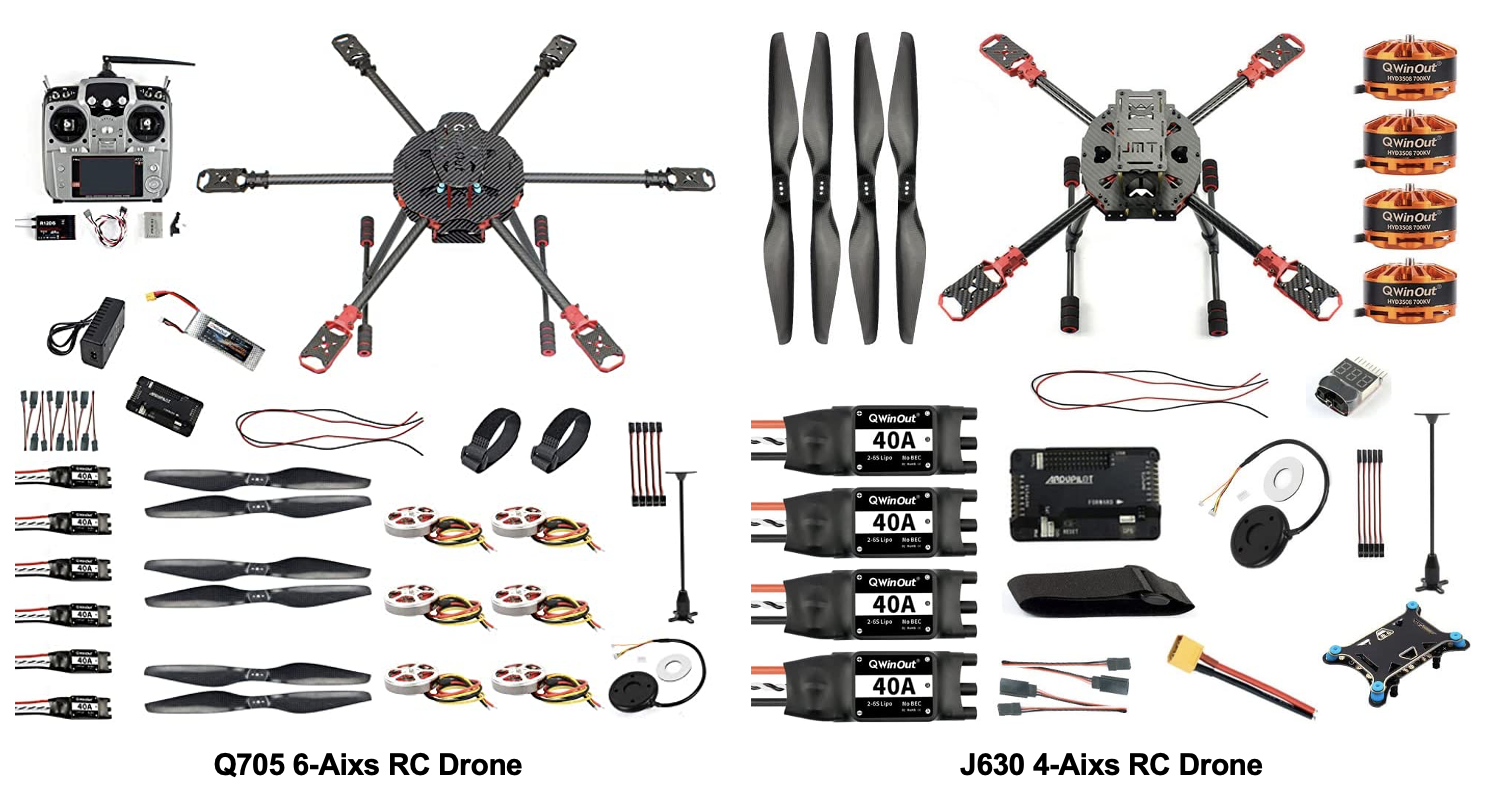
\includegraphics[width=0.5\textwidth]{Figures/Methods/Drone_Kits.png}}
        \caption{(left) 6-Axis RC Drone / (right) 4-Axis RC Drone.}
        \label{fig2a1}
    \end{figure}
    
    There are two types of drones used in the project, as shown in Fig.~\ref{fig2a1}, the larger 6-axis RC drone and the new smaller 4-axis drone purchased in the 2023 spring semester. The larger 6-axis drone is a continuation of the team's work from the previous semester, and the smaller 4-axis drone is a new drone that we assembled in the 2023 spring semester.
    
    \subsubsection{Transistor \& Receiver}\label{subsection:A2}
    \begin{itemize}
        \item SIK Telemetry Radio
        \item Flysky FS-i6   6CH 2.4GHz RC Transmitter
        \item Flysky FS-i6X 10CH 2.4GHz RC Transmitter
        \item iA6B Receiver
        \item iA10B Receiver
    \end{itemize}

    \begin{figure}[H]
        \centerline{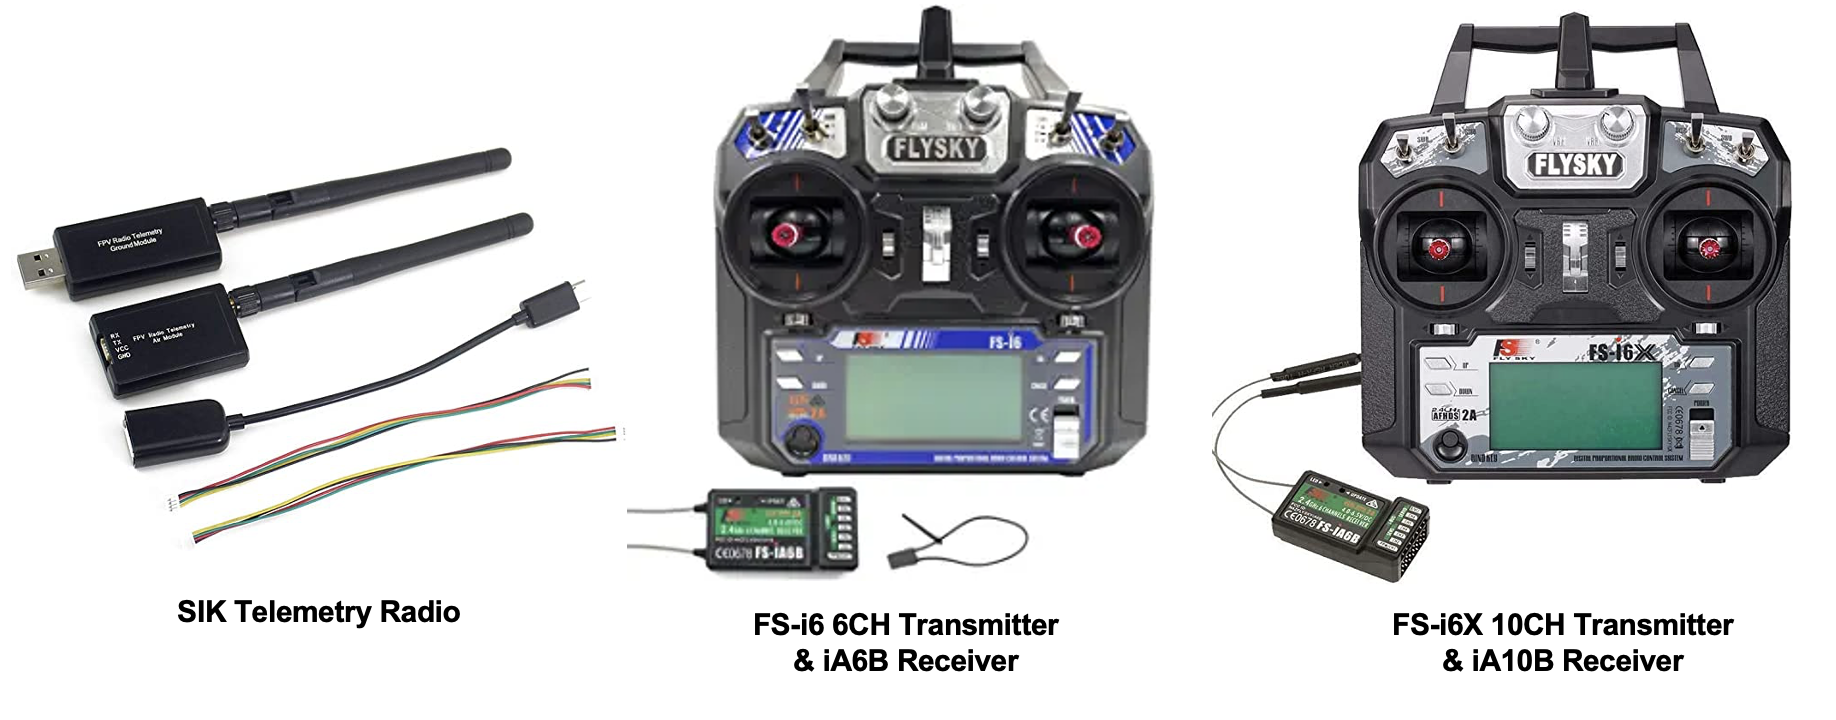
\includegraphics[width=0.5\textwidth]{Figures/Methods/Transistors&Receivers.png}}
        \caption{(left) SIK Telemetry Radio / (middle) FS-i6 6CH Transmitter \& iA6B Receiver / (right) FS-i6X 10CH Transmitter \& iA10B Receiver.}
        \label{fig2a2}
    \end{figure}

    Since we use two types of drones, there are different Transistors \& Receivers for each, as shown in Fig.~\ref{fig2a2}. FS-i6 6CH and iA6B Receiver pairing is for 6-axis drone. FS-i6X 10CH and iA10B Receiver pairing is for 4-axis drone. Then SIK radio just used to communicate between flight controller and Laptop/PC.
    
    \subsubsection{Flight Controller}\label{subsection:A3}
    \begin{itemize}
        \item Cube Black Flight Controller
        \item APM2.8 Flight Controller (Archive)
    \end{itemize}

    \begin{figure}[H]
        \centerline{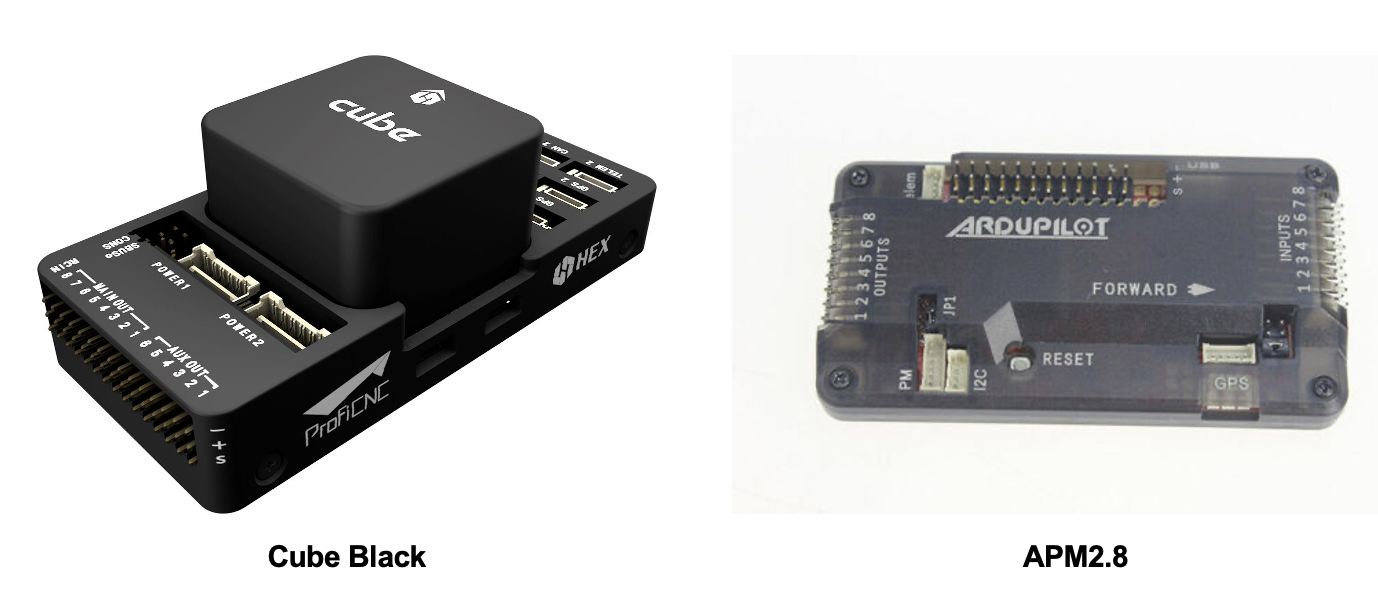
\includegraphics[width=0.5\textwidth]{Figures/Methods/Flight_Controllers.png}}
        \caption{(left) Cube Black / (right) APM2.8.}
        \label{fig2a3}
    \end{figure}

   In the Spring 2023 semester of our project, we employed two flight controller modules, vital for governing the drone's flight and stability. These controllers, processing data from various sensors like accelerometers, gyroscopes, magnetometers, and barometers, ensure optimal altitude, orientation, and movement. Initially, as illustrated in Fig.~\ref{fig2a3}, both the APM2.8 and Cube Black modules were used. However, challenges with calibration and parameter input on the APM2.8 led to its exclusion from the project. Consequently, our focus shifted entirely to utilizing the Cube Black for its superior performance and reliability in flight control operations.
    
    \subsubsection{Embedded System / Controller}\label{subsection:A4}
    \begin{itemize}
        \item Jetson Orin Nano
        \item Raspberry Pi 3B
        \item Raspberry Pi 4B
    \end{itemize}

     \begin{figure}[H]
        \centerline{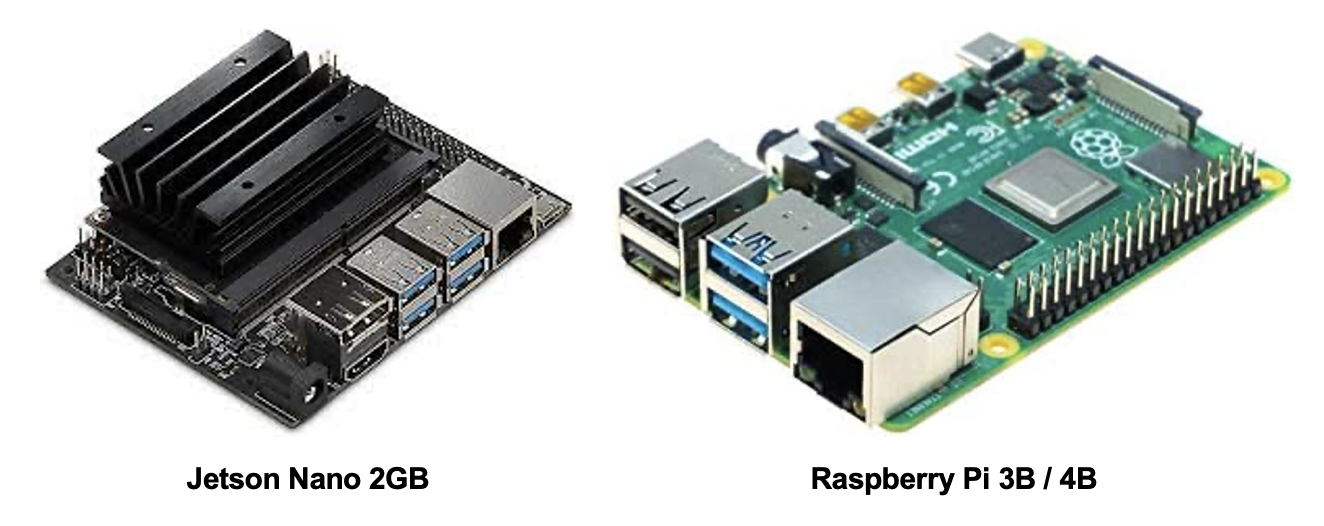
\includegraphics[width=0.5\textwidth]{Figures/Methods/Embedded_Systems.png}}
        \caption{(left) Jetson Orin Nano / (right) Raspberry Pi 3B / 4B.}
        \label{fig2a4}
    \end{figure}

    In the AutoDrone project, our main controller is the embedded system, essential for executing tasks. It captures images from the camera and LiDAR, applying deep learning algorithms for accurate person re-identification and tracking. These algorithms process depth information, guiding the drone's flight controller for precise maneuvering in complex environments.
    
    Our project utilizes two embedded devices: the GPU-equipped Jetson Orin Nano and the smaller Raspberry Pi 3B / 4B, as shown in Fig.~\ref{fig2a4}. We are testing both to assess their compatibility and effectiveness for the project, ensuring optimal performance in real-world scenarios.

    \subsubsection{LiDAR}\label{subsection:A5}
     \begin{figure}[H]
        \centerline{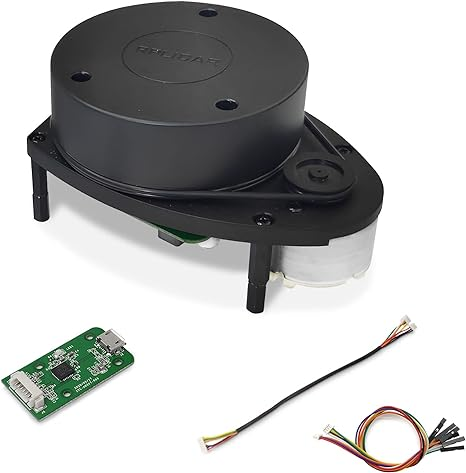
\includegraphics[width=0.2\textwidth]{Figures/Methods/LiDAR.jpg}}
        \caption{LiDAR.}
        \label{fig2a5}
    \end{figure}
    This LiDAR module eas used to detected 2D range around the drone Fig.~\ref{fig2a5}.
\subsection{System Design}\label{subsection:B}

The system consists of essential components, including a Jetson Orin Nano and/or Raspberry Pi to process deep learning models. The Drone-Kit API and MAVLink protocol facilitate communication with the Cube Black flight controller, which ultimately controls the drone's motor and navigation. The system flow chart is depicted in Fig.~\ref{fig2b1}.

Two embedded devices, the Jetson Nano and Raspberry Pi, are incorporated into the drone to compare their performance. Additionally, a SIK radio block is utilized to send the drone's status back to a Laptop/PC for real-time monitoring. For added safety, a Flysky FS-i6 6CH 2.4GHz RC Transmitter and iA6B Receiver are included to enable manual drone control.

    \begin{figure}[H]
        \centerline{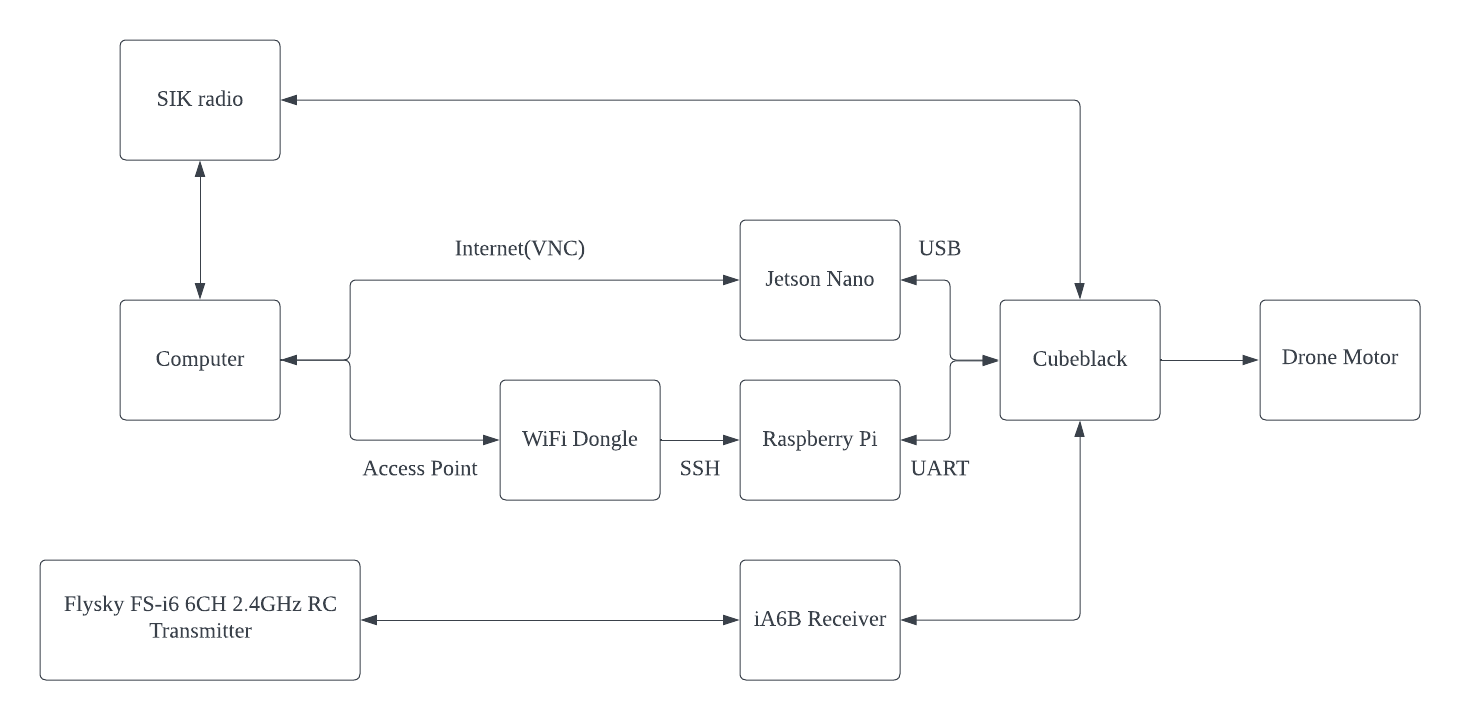
\includegraphics[width=0.5\textwidth]{Figures/Methods/System Flow Chart.png}}
        \caption{System Flow Chart.}
        \label{fig2b1}
    \end{figure}

    \begin{figure}[H]
        \centerline{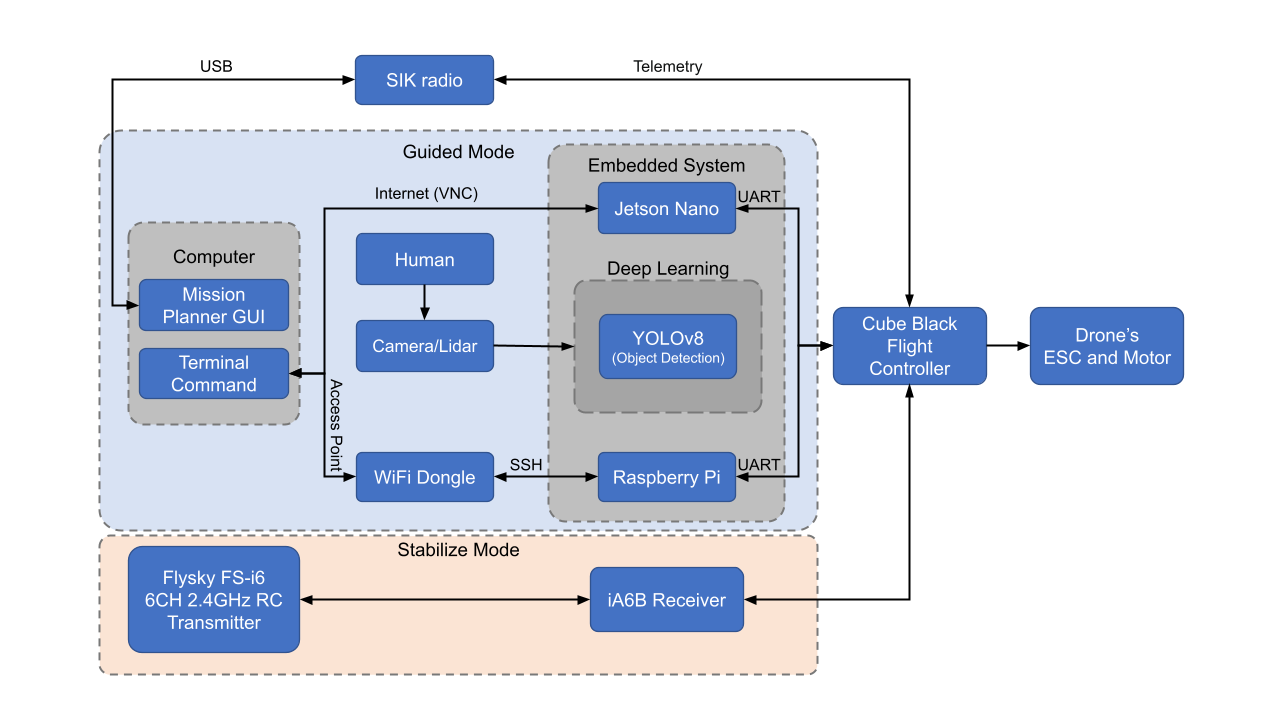
\includegraphics[width=0.5\textwidth]{Figures/Methods/System_Overall_Design.png}}
        \caption{Overall System Design.}
        \label{fig2b2}
    \end{figure}

Fig.~\ref{fig2b2} provides a detailed overview of the system design. The process starts with capturing an image of people using a camera. The image is then analyzed using Deep Learning's YOLOv8 object detection model, which runs on the Embedded System Jetson Orin Nano and/or Raspberry Pi. YOLOv8 is used to detect human in the image (Please note sections \ref{subsection:C} below for more information on YOLOv8), while LiDAR scans for the distance between the human and the drone. (Please note sections \ref{subsection:D} below for more information on LiDAR)


For manual control, we use the Flysky FS-i6 6CH 2.4GHz RC Transmitter in Stabilize Mode, which disables pre-arming checking and puts the drone in an unstable mode. However, to operate the drone using scripts, it must be set to Guided Mode, which allows pre-arming checks to ensure the drone is in a safe condition to complete the pollination task.
\subsection{YOLOv8}\label{subsection:C}
Object detection is a crucial aspect of autonomous drone operation. While there are many deep learning models that can be used for object detection, Convolutional Neural Networks (CNNs) are the most researched method. However, these models mostly use a two-stage pipeline which may not be efficient for autonomous drone purposes. In contrast, one-stage models such as YOLO (You Only Look Once) \cite{2c1} model is a state-of-the-art real-time object detection algorithm, known for its high speed and accuracy. YOLO processes the input image by dividing it into a grid and predicting a set of bounding boxes, objectness scores, and class probabilities for each grid cell. These predictions are combined and subjected to non-maximum suppression to remove overlapping boxes, generating the final object detection. During this semester, our team underwent a significant transition from YOLOv5\cite{2c2} to the latest iteration, YOLOv8\cite{2c3}, in our pursuit of advancing object detection and segmentation capabilities. The model is built on a foundation of extensive pre-training on millions of images and places a particular emphasis on its zero-shot learning capabilities.

In our AutoDrone Re-ID project, our primary focus is on the detection of people using a webcam mounted on the drone. The YOLOv8 model assumes a crucial role in identifying individuals within the camera frame, thereby enhancing the overall efficiency and safety of the drone's operation. The YOLOv8 model is implemented using the PyTorch framework, offering a diverse selection of pre-trained models, each striking a unique balance between speed and accuracy. Our team opted for the YOLOv8s model, a more compact version with a parameter count of 11.2 millions. This strategic decision ensures optimal performance within the limitations of the drone's hardware.

In the context of our AutoDrone project, the YOLOv8 model has successfully demonstrated several key functionalities. Utilizing the YOLOv8 model, our implementation enables precise people counting in a given scene over a specified period. This capability facilitates the comprehensive analysis of crowd dynamics, providing valuable insights for operational decision-making. Furthermore, in alignment with the global emphasis on safety measures, our YOLOv8 model has been enhanced to incorporate mask detection capabilities by trained with a random sample of MaskedFace-Net dataset\cite{2c4}. It can accurately identify individuals, distinguishing between those wearing masks and those without, thereby adding an extra layer of safety in public spaces.
\subsection{Camera, LiDAR, and FCU}\label{subsection:D}
% TODO: add a section for lidar

First, the implementation of the Robot Operating System (ROS) on the Jetson Orin Nano involved a detailed process of hardware and software setup. This setup was fundamental for installing ROS libraries and configuring the operating system to support the demands of real-time robotic control. A key aspect of this implementation was the development of custom ROS nodes. These nodes were designed to perform specific functions such as data acquisition, processing, and transmission of commands. They were capable of publishing and subscribing to topics within the ROS environment, facilitating a dynamic data exchange system.

Next, various sensors were integrated, including cameras, GPS, IMUs, and LiDAR into the ROS framework, this required the development of custom drivers and interfaces to ensure a seamless flow of data from the sensors into the ROS system. In parallel, a robust connection between the Jetson Orin Nano and the drone's flight control unit was established using MAVROS and MAVProxy. MAVROS acted as a bridge, enabling real-time communication and command exchange. A link with this protocol was set up for transmitting control commands from the ROS nodes to the drone and for receiving flight data from various sensors in the flight control unit.

Then, to enhance the drone's sensory capabilities, the drone involved mounting additional cameras and LiDAR \cite{2d1}, as shown in Fig. ~\ref{fig2d1}. The placement of these sensors was strategically chosen to optimize the field of view and depth perception. An important step in this process was the calibration of the sensors to ensure accuracy in data capture. Algorithms were then developed to merge data streams from these cameras and Lidar. This fusion created a comprehensive view combining both image and depth information, essential for advanced perception. To ensure efficiency, the optimized image capture package V4L was employed instead of openCV to minimize latency in data transfer and processing. RVIZ, a visualization tool within ROS, was customized for real-time monitoring and debugging of the fused data. This setup facilitated a clear visualization of how image and depth data were combined, aiding in system refinement and development.
    \begin{figure}[H]
        \centerline{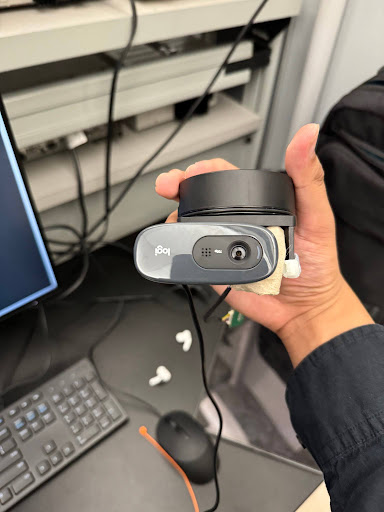
\includegraphics[width=0.3\textwidth]{Figures/Methods/physical_setup.jpg}}
        \caption{Physical Setup of the Camera and Lidar}
        \label{fig2d1}
    \end{figure}
The project focused on developing algorithms for obstacle avoidance, tracking, person detection, and counting. These algorithms were designed to utilize the data provided by the integrated sensors, enabling the drone to dynamically interact with its environment. Gazebo, a robotic simulator was heavily used in testing these algorithms, as shown in Fig. ~\ref{fig2d2}. It provided a controlled environment to simulate various scenarios, allowing for the fine-tuning of algorithms before real-world application. By setting up the obstacles in the simulated world, the drone's obstacle avoidance function can be tested by letting the drone found its own way out in a maze. This process involved the use of Lidar and the motion control of the drone.

    \begin{figure}[H]
        \centerline{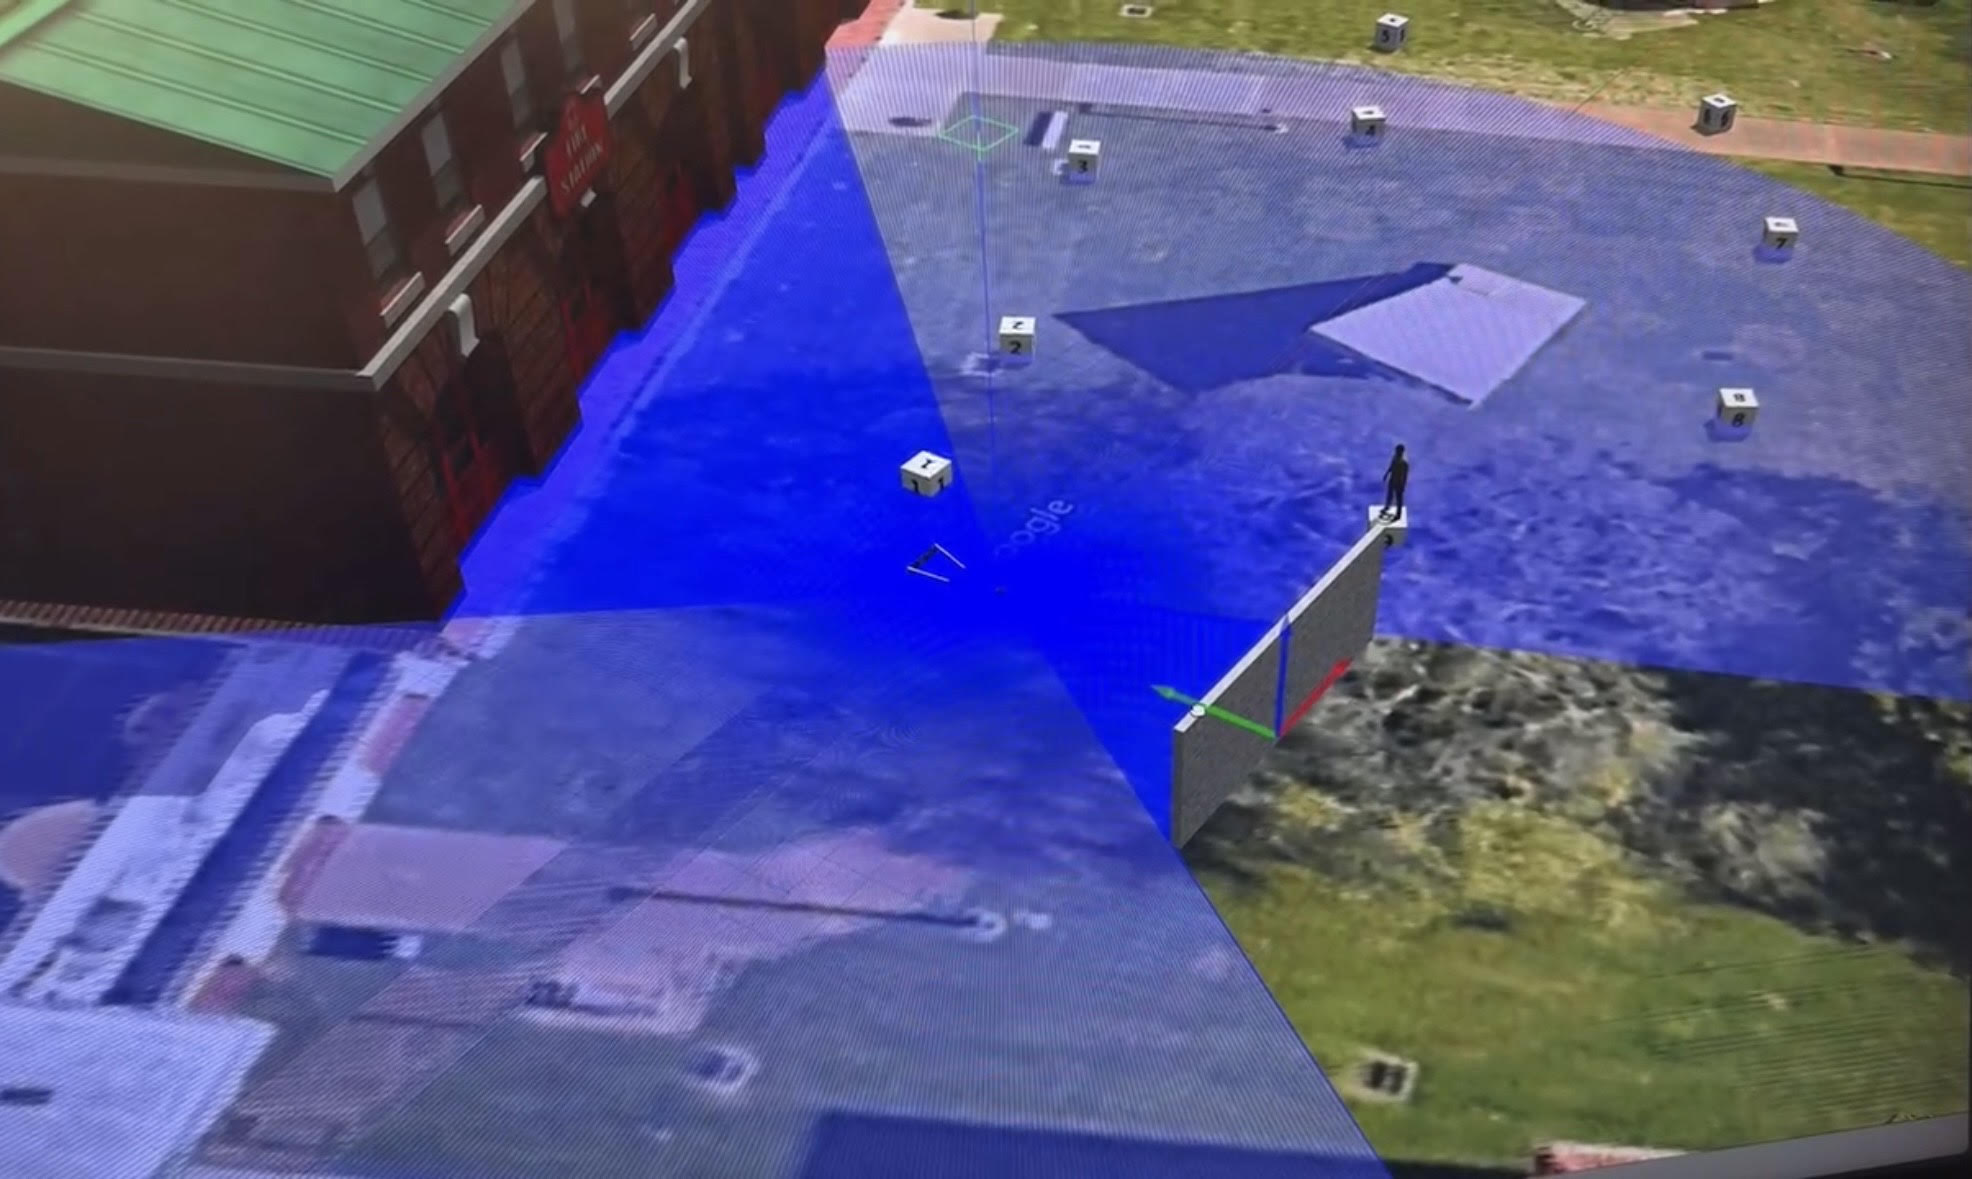
\includegraphics[width=0.5\textwidth]{Figures/Methods/gazebo_lidar.jpg}}
        \caption{Scenario Setup in Gazebo}
        \label{fig2d2}
    \end{figure}
    
Finally, the data collection and analysis during these simulations were vital in assessing and optimizing the performance of the algorithms. This iterative process involved making adjustments based on performance metrics to enhance efficiency and accuracy. Once the algorithms were satisfactorily developed and tested in the simulator, they were integrated into the ROS environment. This integration entailed coding the algorithms into ROS nodes and ensuring they interacted seamlessly with other system components. Preliminary field tests were then conducted to evaluate the performance of these algorithms in real-world conditions, with observations from these tests used to make further adjustments and improvements.

\subsection{Software in the Loop (SITL)}\label{subsection:E}
In executing the SITL simulation, a detailed virtual environment was established in the Gazebo simulator to closely mimic real-world conditions. This environment included models like buildings and trees, sourced directly from the Gazebo library. Additionally, to recreate an accurate geographical setting, a plane was generated using satellite imagery from the Google Maps API \cite{2e1}. This incorporation of real-world geographic data and physical objects greatly improved the authenticity of the simulated environment.

Additionally, human models were crafted using MakeHuman, a sophisticated tool designed to create realistic human avatars, and were subsequently rendered with Blender software. The files exported from MakeHuman included a mesh model, texture images, and a UV map — which is a flat representation of the 3D model used to map textures. All these components were imported into Blender to produce the final 3D rendered model. A demonstration of the human model creation process using MakeHuman and Blender is presented in Figure ~\ref{fig2e1}. This method provided lifelike representations of humans, which is essential for the drone's person re-identification capabilities.


\begin{figure}[H]
    \centerline{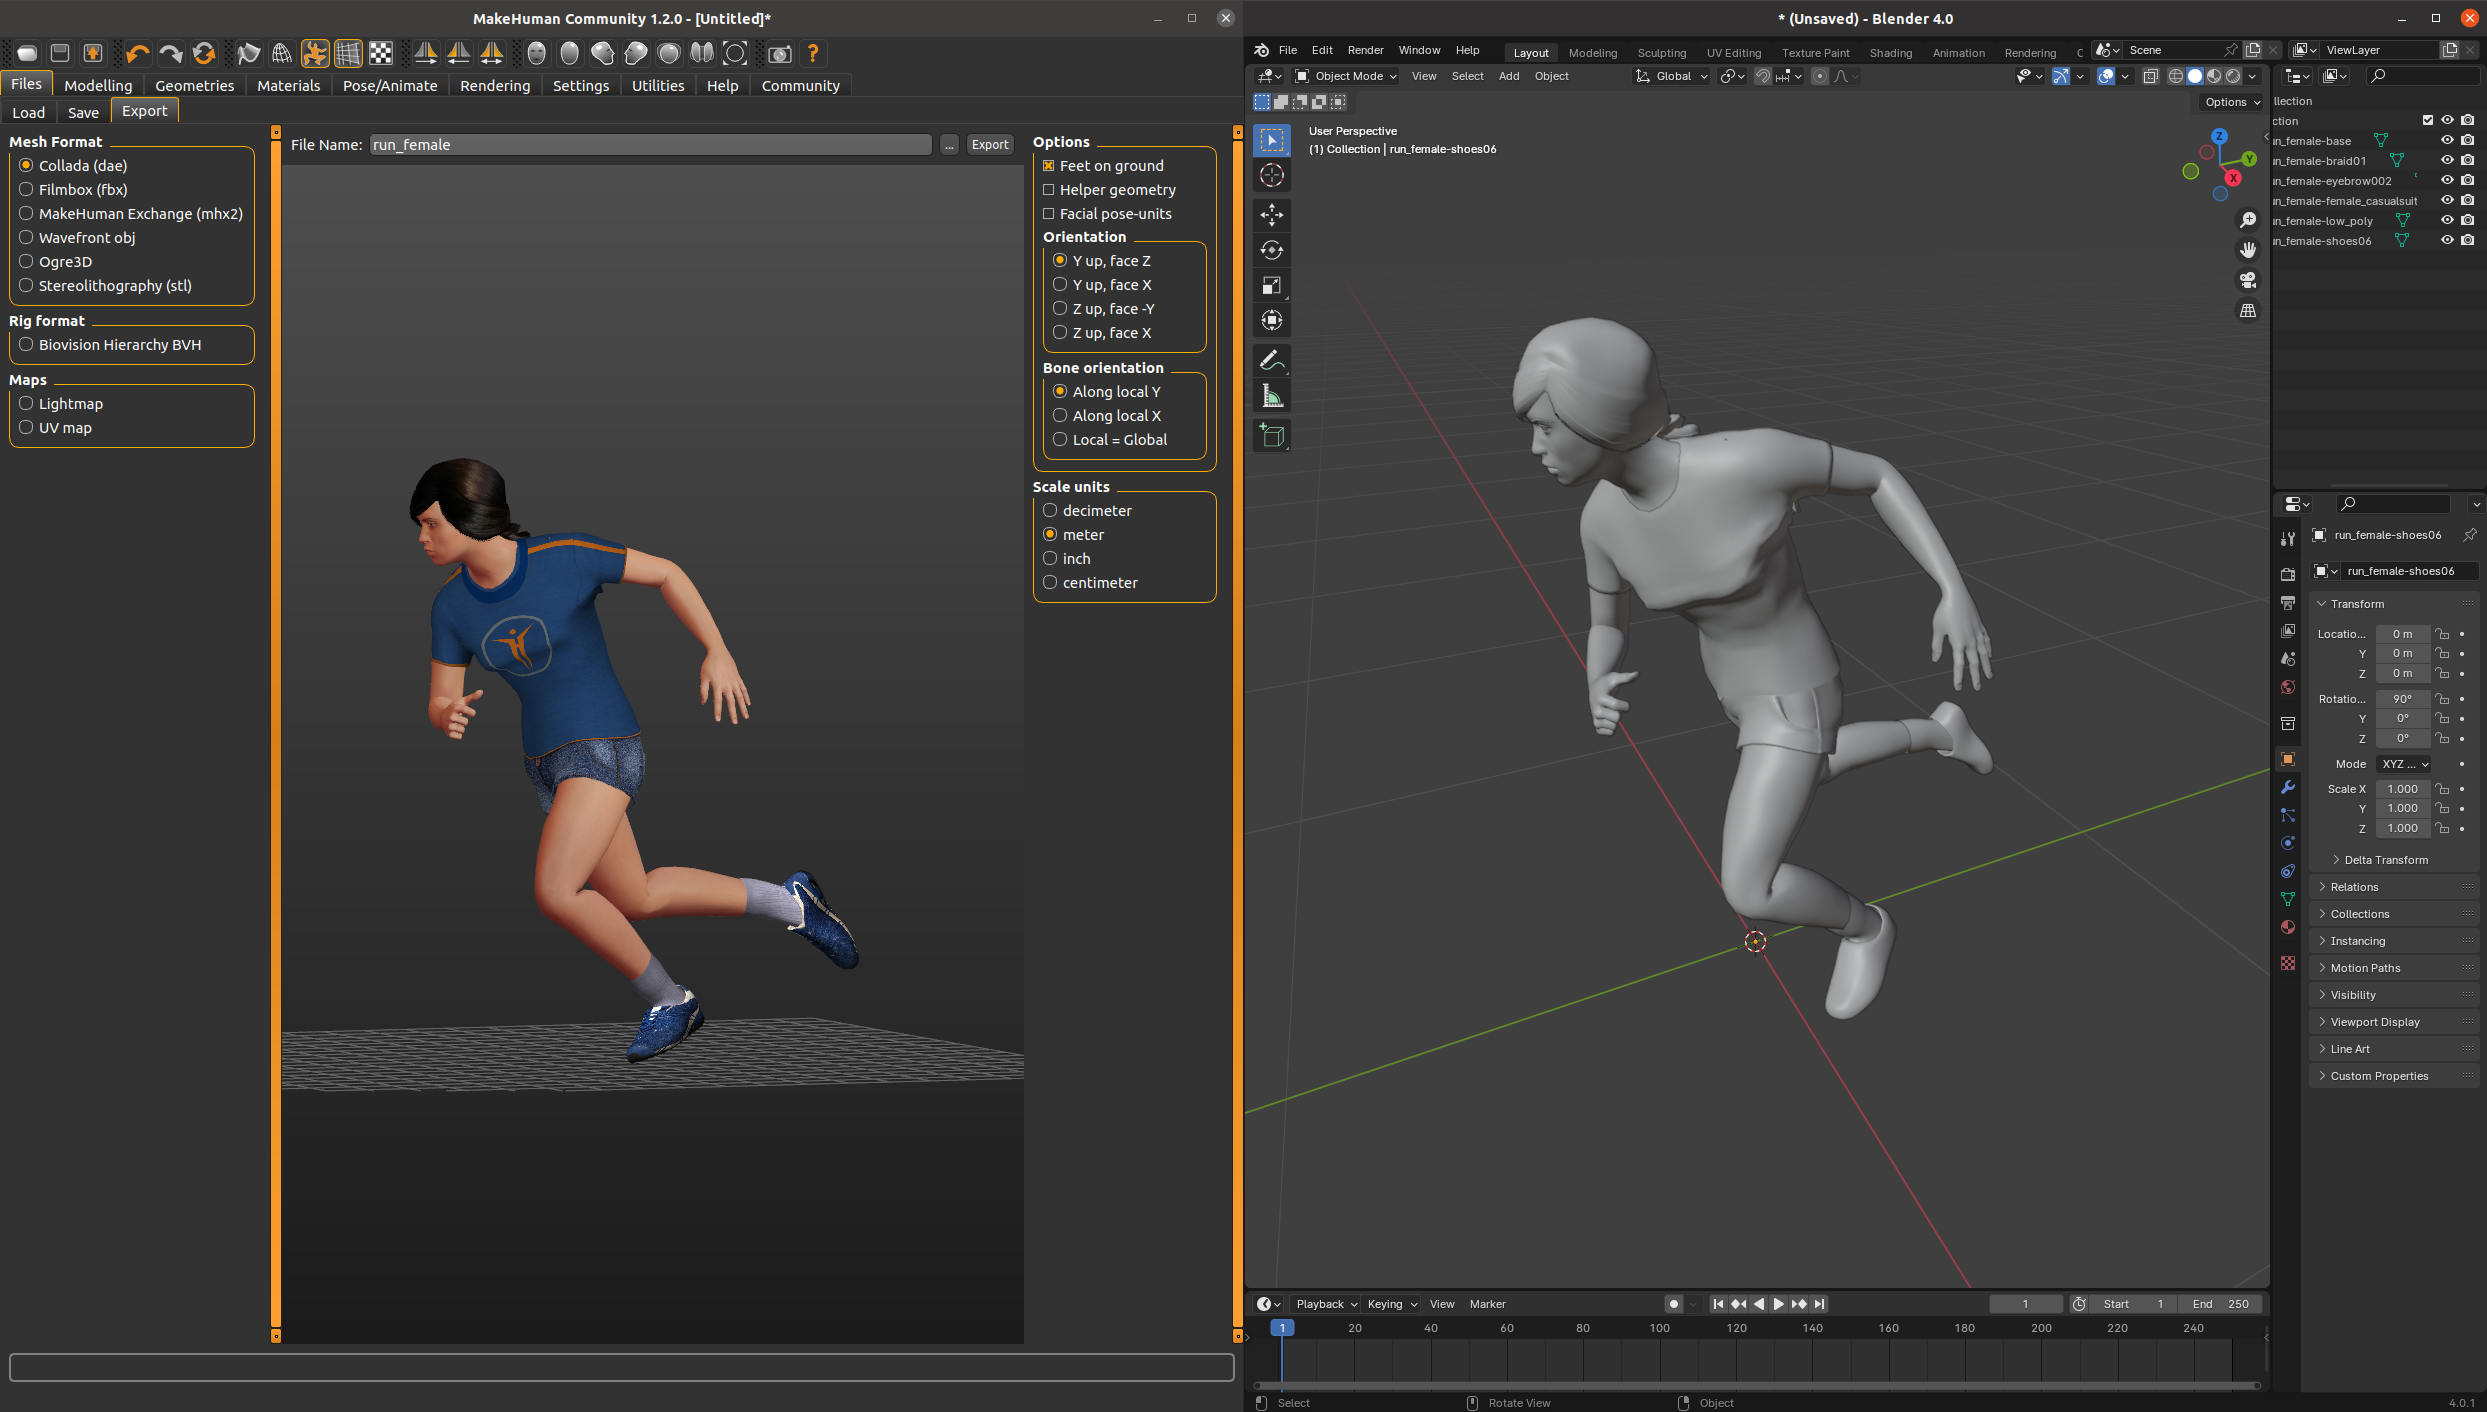
\includegraphics[width=0.5\textwidth]{Figures/Methods/makehuman+blender.png}}
    \caption{Human Model Creation Process: (left) MakeHuman / (right) Blender}
    \label{fig2e1}
\end{figure}

The centerpiece of the simulation was the Iris quadcopter model, equipped with a camera and a LiDAR sensor. The integration of these sensors into the Iris quadcopter model was crucial for the autonomous drone to navigate and recognize humans within the simulated environment accurately. A sample of the fully integrated world is illustrated in Figure \ref{fig2e2}.   

\begin{figure}[H]
    \centerline{\includegraphics[width=0.5\textwidth]{Figures/Methods/env.png}}
    \caption{Gazebo World Environment}
    \label{fig2e2}
\end{figure}

Ardupilot's SITL is essential in the setup of the simulation for the project. It simulates the flight control hardware for the quadcopter in Gazebo and establishes a bridge to the ROS environment. The block diagram shown in Figure \ref{fig2e3} illustrates the communication pathway between the drone's Flight Control Unit (FCU) within Ardupilot's SITL and the Gazebo simulation environment, facilitated by the Gazebo Driver and MAVProxy. Gazebo handles the simulation of the drone's physical responses and sensor inputs, which are then interfaced with the ROS environment through ROS topics. ROS, in turn, sends control signals to the FCU using the MAVLink protocol via UDP ports. This process coordinates the drone's simulated activities and completes the loop of the integrated simulation system.

\begin{figure}[H]
    \centerline{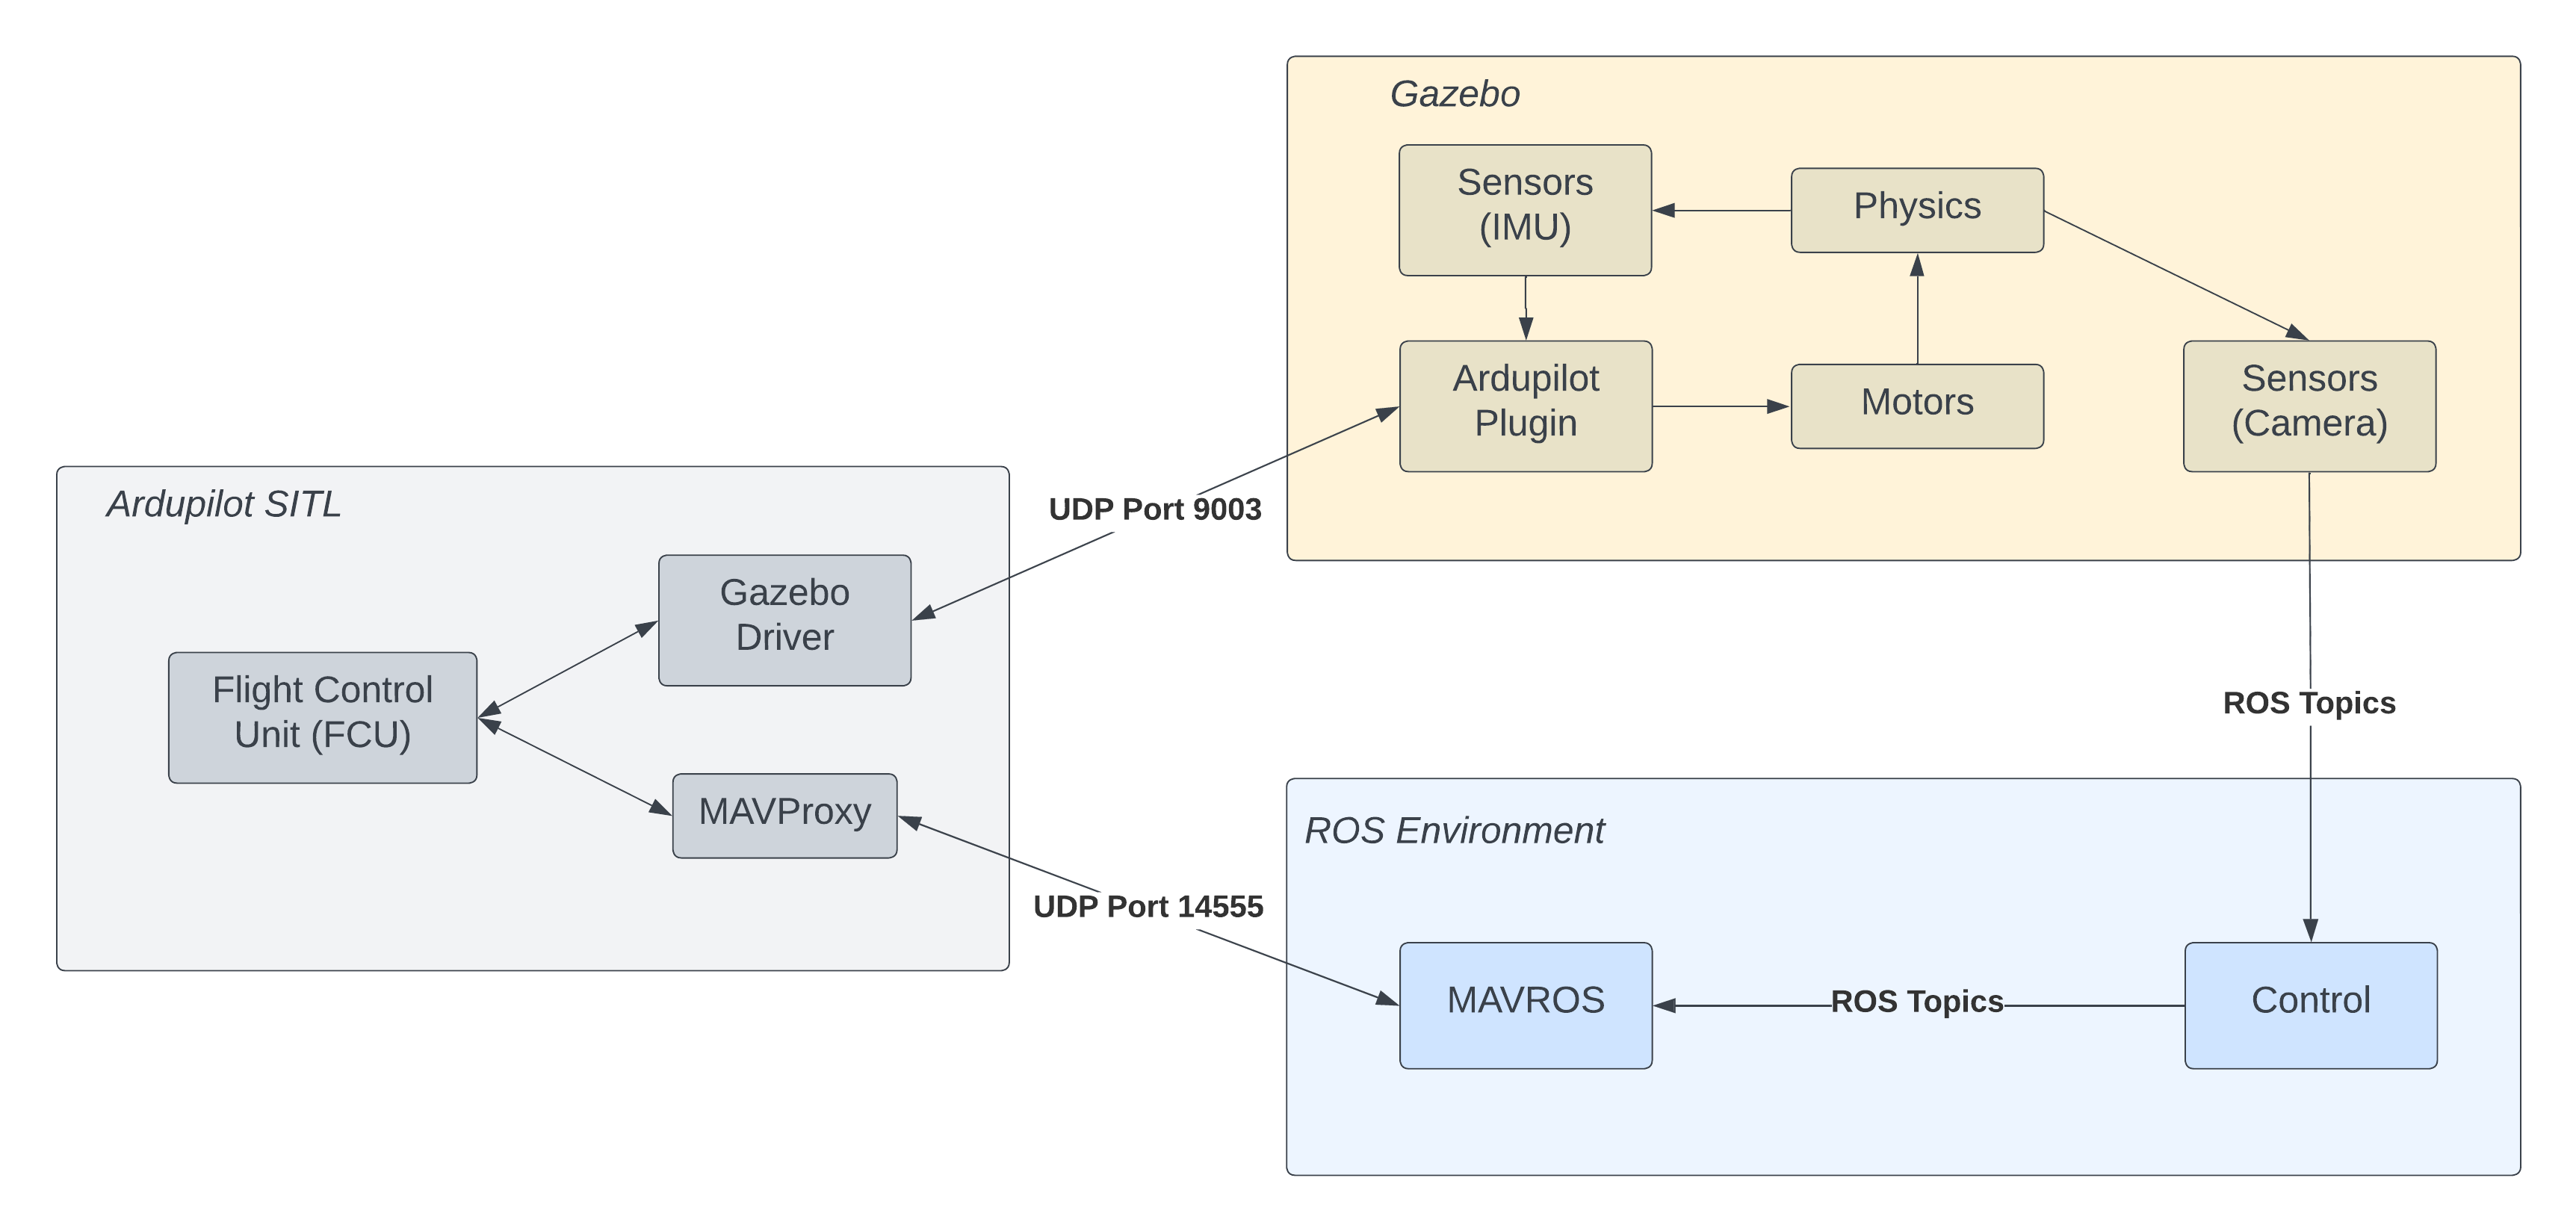
\includegraphics[width=0.5\textwidth]{Figures/Methods/sitl_block_diagram.png}}
    \caption{SITL Block Diagram}
    \label{fig2e3}
\end{figure}

In developing the autonomous drone's control and object detection functionalities, specific libraries were selected for optimal performance and system compatibility. The "gnc\textunderscore functions" library from Intelligent Quads was chosen for drone control\cite{2e2}. It provides a comprehensive set of guidance, navigation, and control (GNC) functions made for autonomous drones, which enables precise maneuvering and stable flight. For object detection, the OpenCV deep neural network (DNN) module was used. The shift from Python to C++ for enhanced performance led to the selection of OpenCV's DNN module, which is well-suited for C++ environments. This module, particularly effective in real-time object detection, was utilized to load the ONNX YOLO model.


The integration of various simulation tools and models played a key role in developing a robust and realistic testing environment for the autonomous drone. This foundation is crucial for the drone's successful application in real-world scenarios.
\subsection{UI}\label{subsection:F}
To monitor the drone's status in real-time, we utilize the SIK Telemetry Radio and Mission Planner GUI. This eliminates the need to develop a complex GUI interface and provides detailed drone status information.
\section{Results}

\subsection{Raspberry Pi Integration}

\begin{figure}[H]
    \centerline{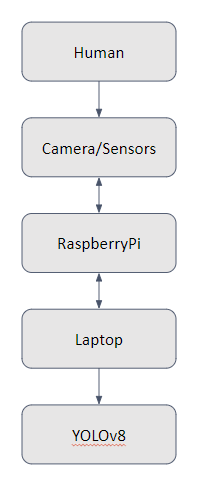
\includegraphics[width=0.1\textwidth]{Figures/Results/Object Detection.png}}
    \caption{Object Detection Flow Chart.}
    \label{fig3a1}
\end{figure}

Fig. ~\ref{fig3a1} shows the flowchart of our object detection with the Raspberry Pi embedded system. As you can see the sequence in the flowchart is by streaming video to Laptop via Raspberry Pi and use YOLOv8 to detect Human.

\begin{figure}[H]
    \centerline{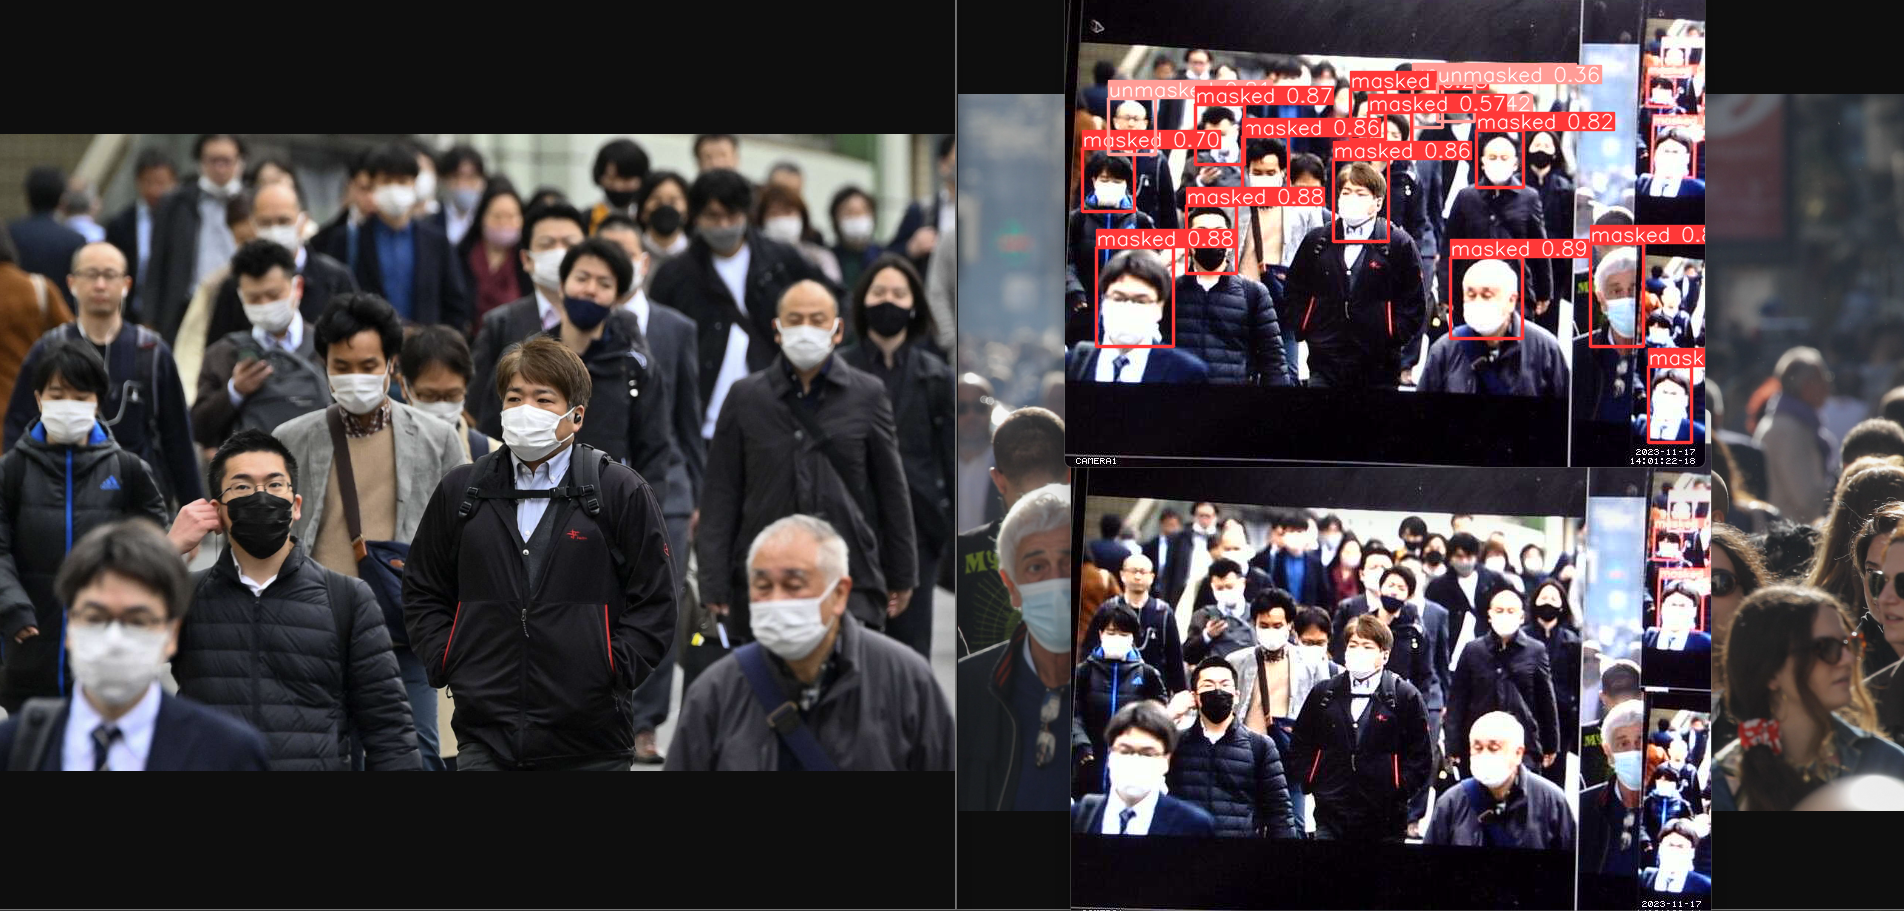
\includegraphics[width=0.5\textwidth]{Figures/Results/RPi_YOLOv8.png}}
    \caption{YOLOv8 model test on real-world dataset with Raspberry Pi 3B.}
    \label{fig3a2}
\end{figure}

Fig. ~\ref{fig3a2} shows the results of real-world dataset testing on the Raspberry Pi 4B using the YOLOv8 model. It can be found that the accuracy is considerable.

As we  we can clearly see the performance differences among them, 
As shown in TABLE \ref{tab1} was the performance difference we had with running Yolov5 on Raspberry Pi 3B, Raspberry Pi 4B. We kept this table here as a referenece and record.
\begin{table}[H]
    \caption{Performance Comparison on running Yolov5}
    \begin{center}
        \resizebox{0.35\textwidth}{!}{%
            \begin{tabular}{|c|c|c|c|}
                \hline
                \textbf{}&\multicolumn{2}{|c|}{\textbf{Controller}} \\
                \cline{2-3} 
                \textbf{Rubric} & \textbf{\textit{RPi3}}& \textbf{\textit{RPi4}} \\
                
                \hline
                CPU (GHz) & 1.2 & 1.5  \\
                \hline
                RAM (GB) & 1 & 8  \\
                \hline
                RAM Usage (MB) & 340 & 332  \\
                \hline
                yolov5s.pt (fps) & 0.21 & 0.95  \\
                \hline
                yolov5n.pt (fps) & 0.43 & 1.67  \\
                \hline
                Load Speed & Very & Very  \\
                (from cmd to start detect) & slow & fast  \\
                
                \hline
            \end{tabular}
        }
        \label{tab1}
    \end{center}
\end{table}

We are also able to control the drone to take off, hover, move in direction, rotation, and landing through Raspberry Pi.
\subsection{Jetson Orin Nano Integration}

This section is from the spring 2023 semester. During the integration of the Jetson Orin Nano and the drone system, we encountered unexpected issues and device malfunctions, which prevented us from incorporating the YOLOv5 detection model and MiDaS depth estimation model into the system. Instead, we utilized the OpenCV library and developed a QR code tracking script that enables the drone to detect QR codes and rotate to track them. 

\begin{figure}[H]
    \centerline{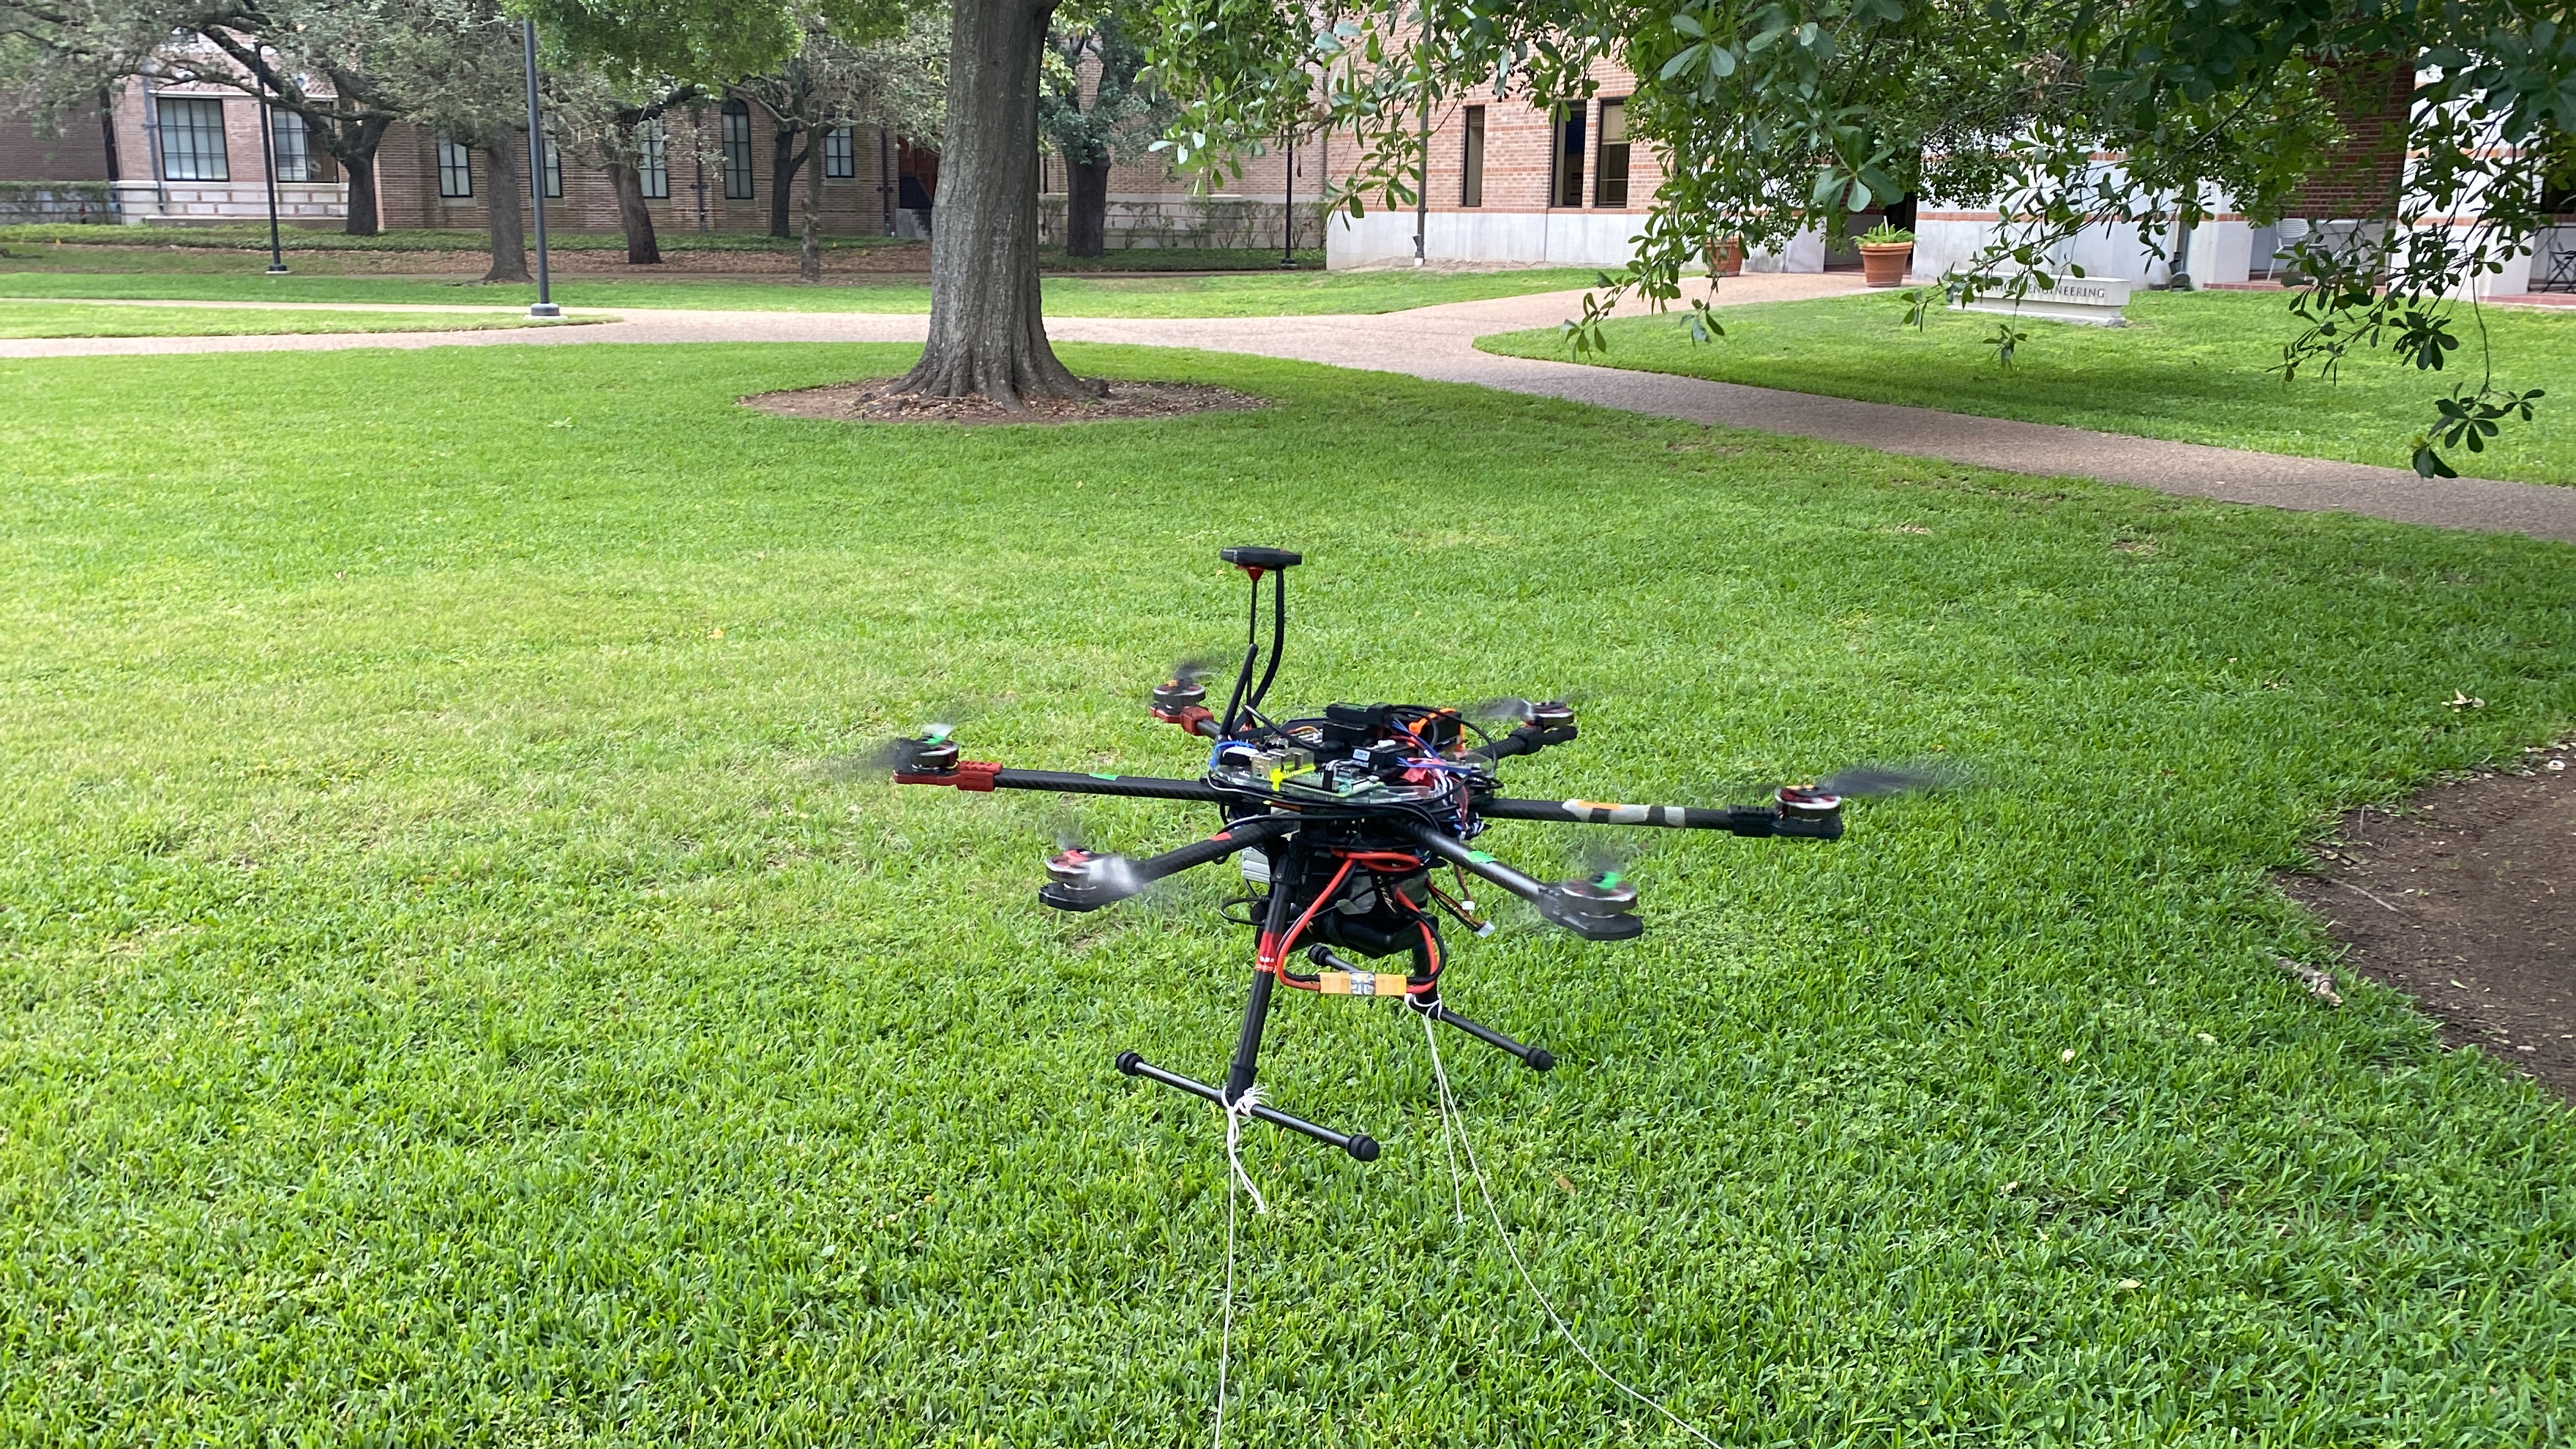
\includegraphics[width=0.5\textwidth]{Figures/Results/Drone_Hover.JPG}}
    \caption{Hover drone in the air operated by Jetson Orin Nano.}
    \label{fig3b1}
\end{figure}

Before implementing this experiment, we tested several other simple movement scripts. Fig. ~\ref{fig3b1} shows the drone hovering successfully in the air for the first time, while Fig. ~\ref{fig3b2} shows the final experiment in which the drone hovers in the air and tracks the QR code. This experiment was conducted in a real-world environment.

\begin{figure}[H]
    \centerline{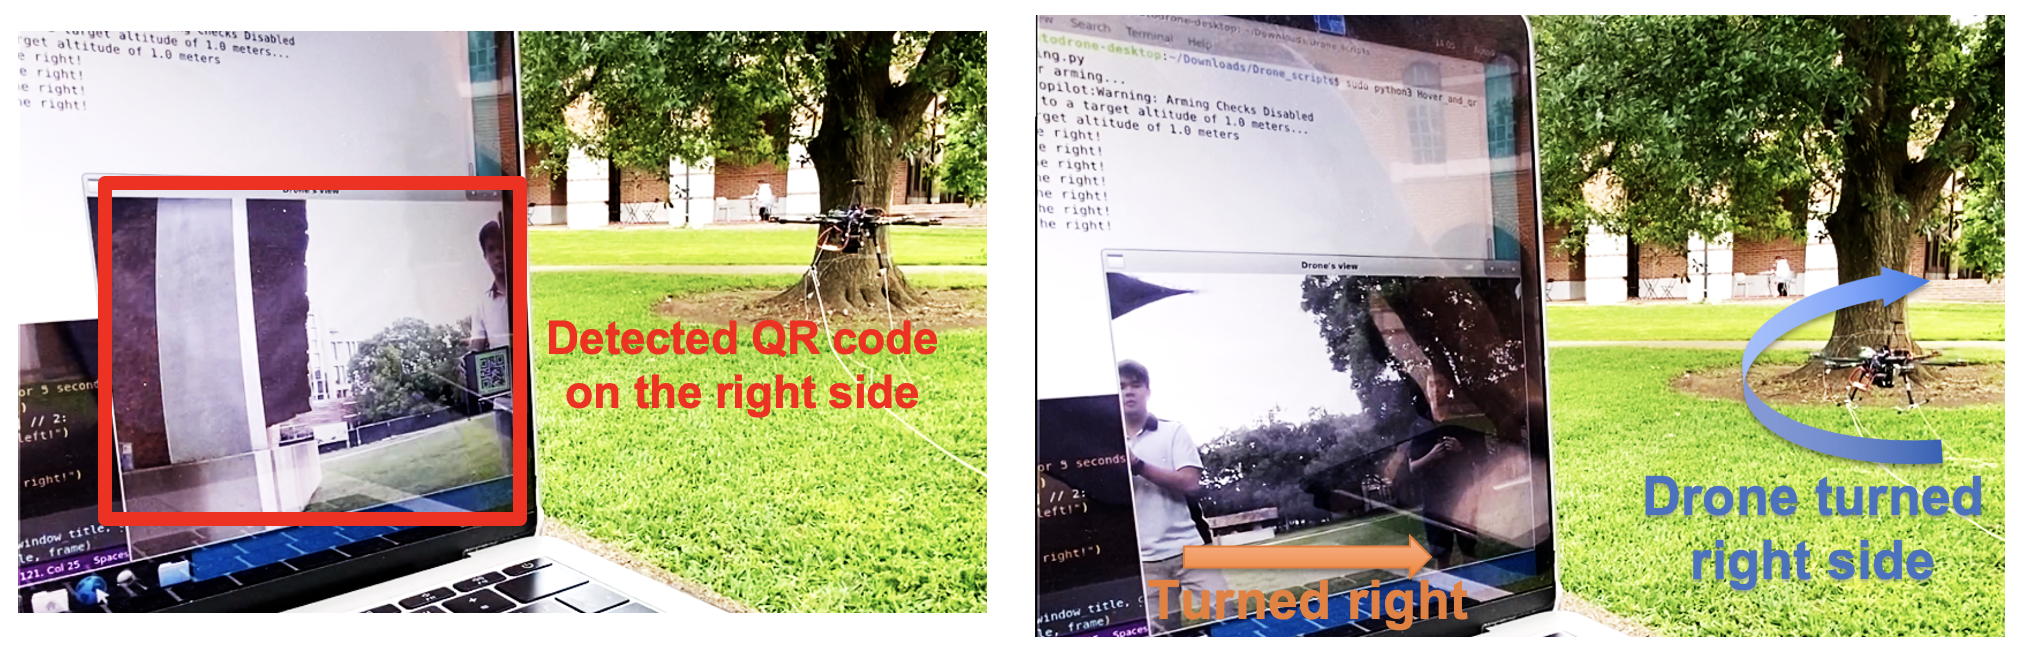
\includegraphics[width=0.5\textwidth]{Figures/Results/QR_code_Tracking_Successfully.png}}
    \caption{QR code tracking results on Jetson Orin Nano.}
    \label{fig3b2}
\end{figure}

This section below is from the fall 2023 semester.
% TODO: Add Stuff

For this semester, the Robot Operating System (ROS)  was successfully integrated in the Jetson Orin Nano, establishing a robust connection with the Ardupilot Flight Control. This integration enabled the comprehensive control and monitoring of the drone system, laying a foundational framework for advanced drone operations. This integration enabled the accessibility and functionality of both external (camera, LiDAR) and internal (GPS, IMU, barometer) sensors within the flight control unit. These sensors now effectively contribute fundamental flight and awareness data to the system. Additionally, the project made strides in enabling motion control of the drone through ROS nodes, facilitated by the effective communication between the Jetson Orin Nano and the flight control unit via MAVROS/MAVPROXY. However, the current motion control system is somewhat limited by the constraints of existing wrapped functions, highlighting an area for future improvement. The project team anticipates enhancing this aspect by developing custom functions using underlying FCU code for more direct interaction with the flight control system.

The project also achieved considerable success in the area of multiple sensor fusion. The integration of camera and lidar sensors was not only successfully accomplished but also optimized to ensure efficient data streaming to ROS topics. This development provided the drone with basic yet powerful perception capabilities. This fusion effectively combined environmental imaging with depth estimation, offering a more comprehensive understanding of the drone's surroundings, as shown in Fig. ~\ref{fig3b3} and  
Fig. ~\ref{fig3b4}. Additionally, the team managed to establish and visualize the spatial orientation of the sensors relative to the drone body using RVIZ, thereby enhancing the drone's spatial awareness by rearranging the transformation between the frames. A significant reduction in the latency of data capture was achieved by transitioning to more efficient capture packages. The project aims to further refine the range and angle mapping between the camera and lidar sensors and develop additional applications to enhance the drone's perception capabilities.

\begin{figure}[H]
    \centerline{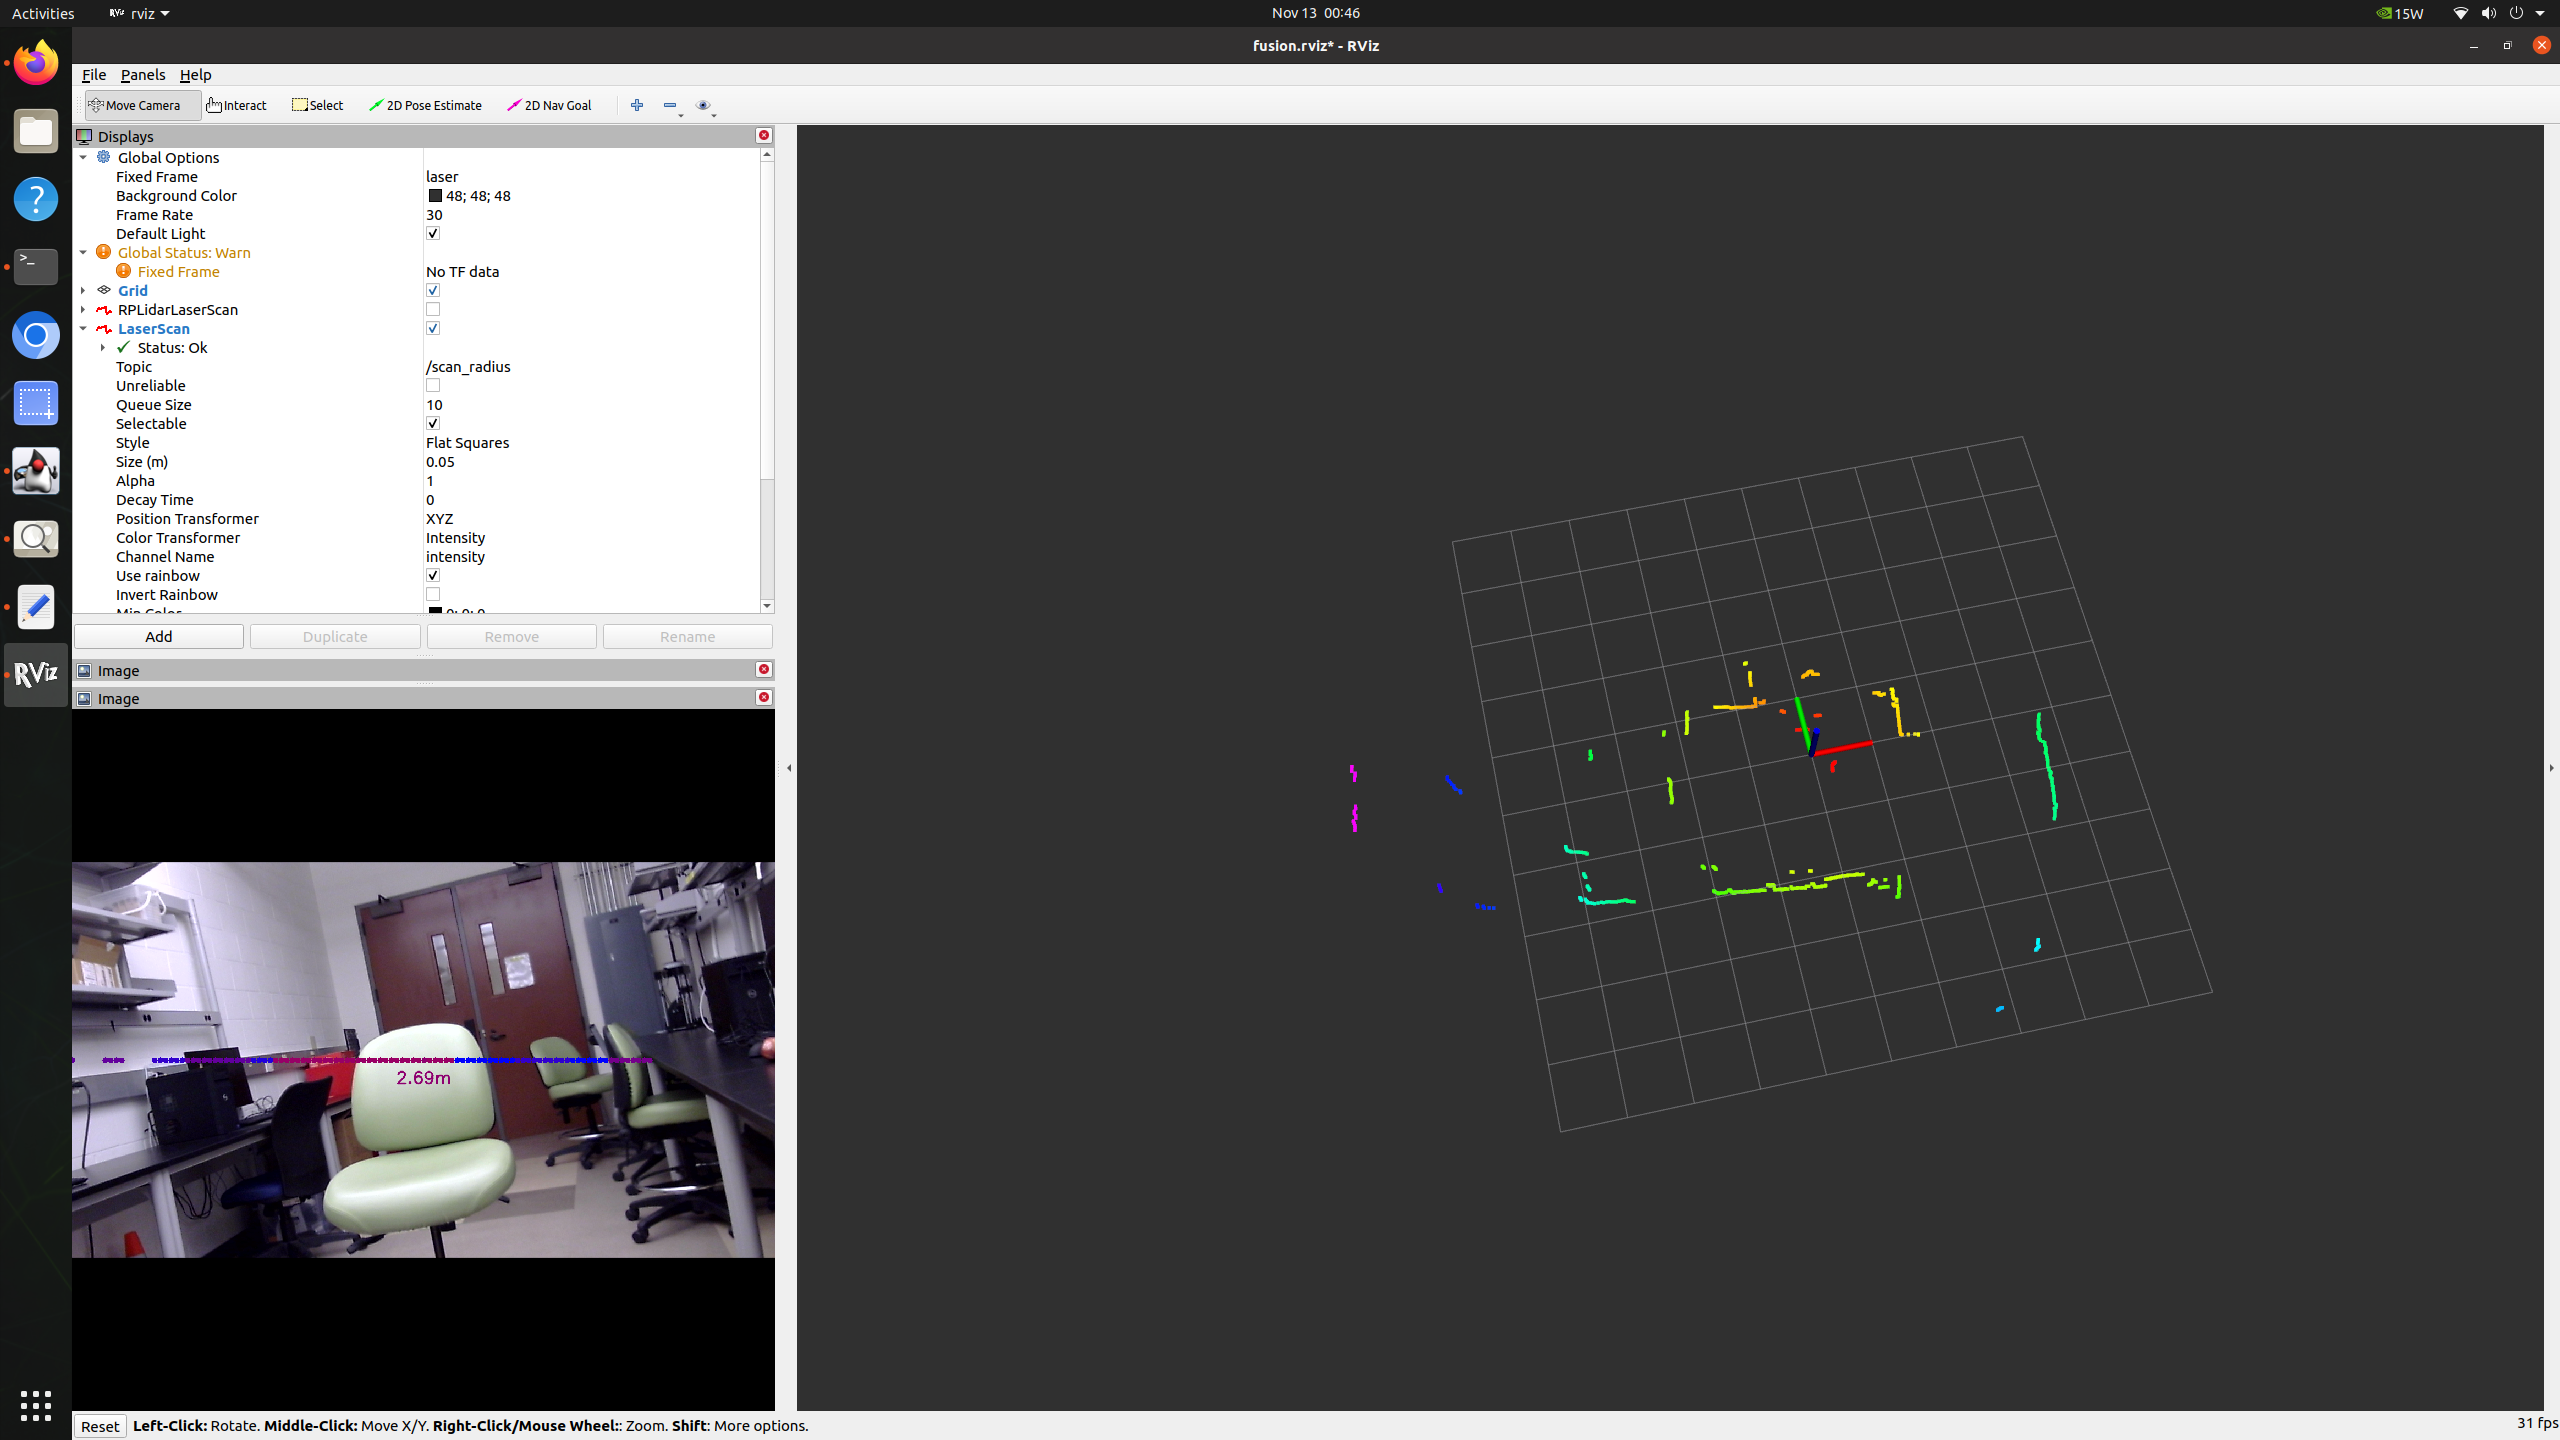
\includegraphics[width=0.5\textwidth]{Figures/Results/fusion5_with_distance.png}}
    \caption{Camera-LiDAR Fusion with Distance Estimation(Close).}
    \label{fig3b3}
\end{figure}


\begin{figure}[H]
    \centerline{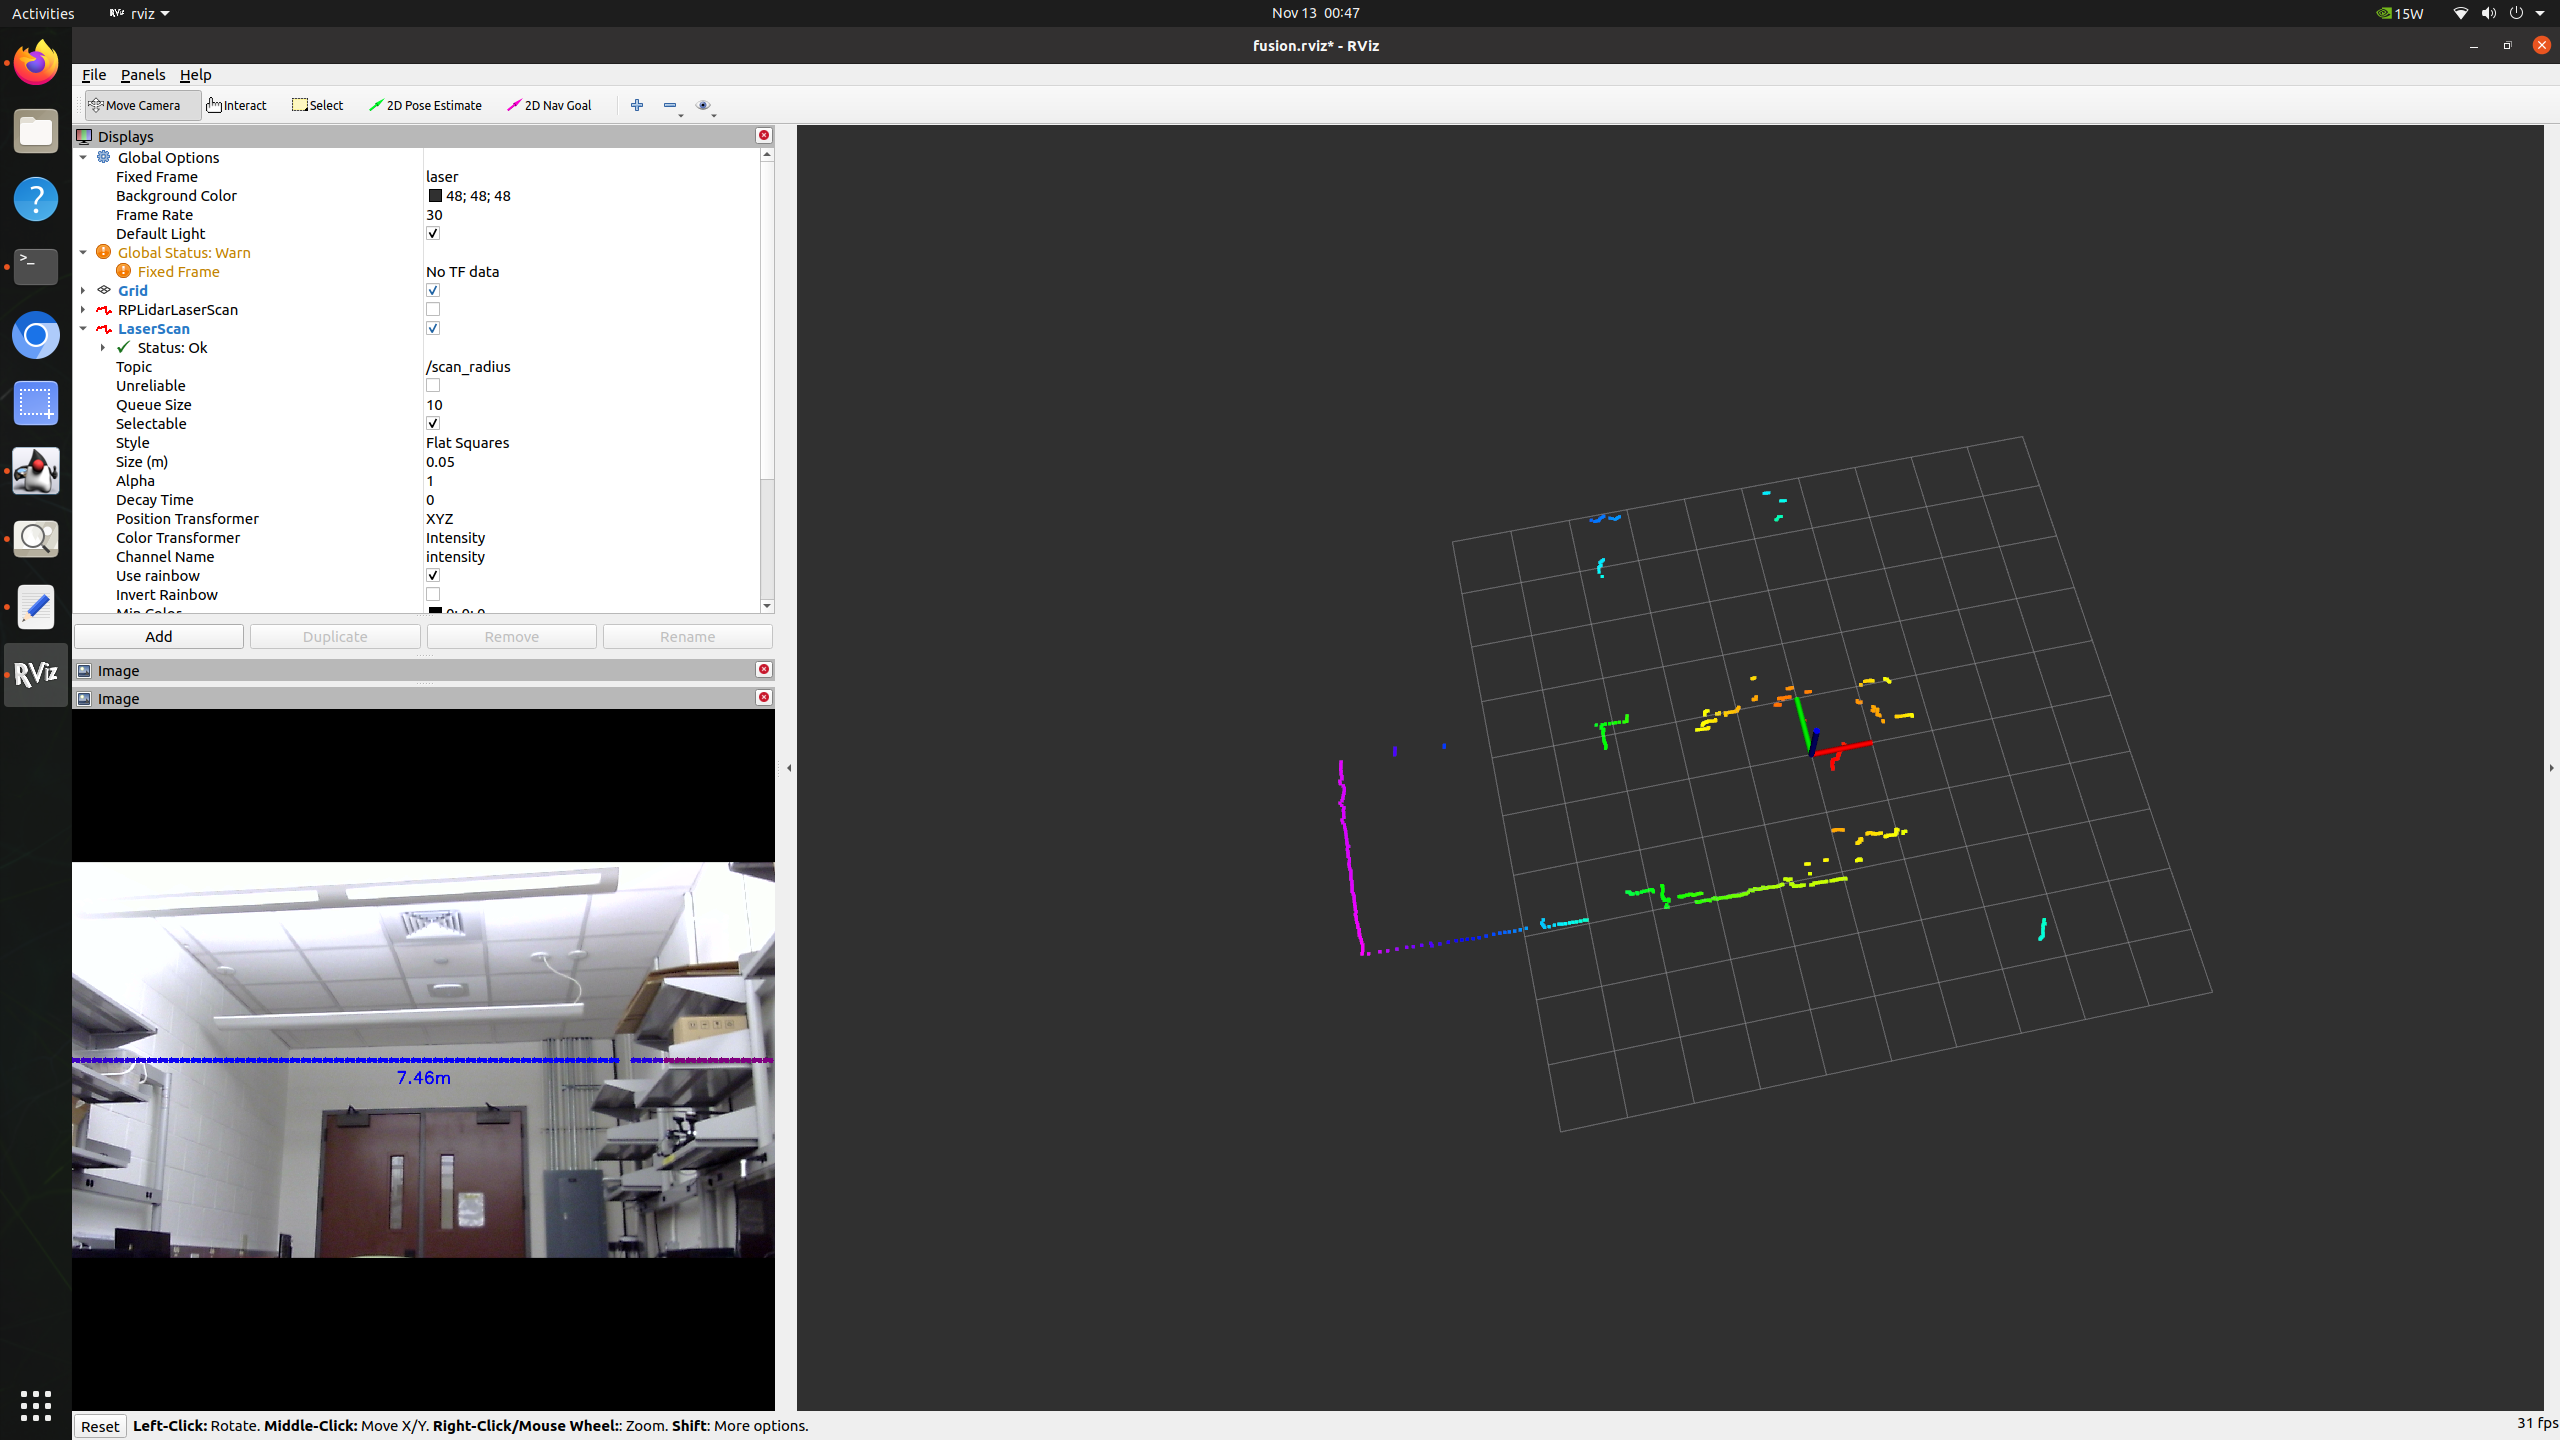
\includegraphics[width=0.5\textwidth]{Figures/Results/fusion6_with_distance.png}}
    \caption{Camera-LiDAR Fusion with Distance Estimation(Far).}
    \label{fig3b4}
\end{figure}

In the realm of on-board algorithm development, the project made substantial progress, aligning closely with initial objectives, although some areas still under development. The obstacle avoidance and tracking algorithms, critical for the drone's navigation and environmental interaction, were developed and tested in a simulator. These preliminary versions demonstrated basic environmental awareness, but full functionality is pending due to a limited understanding of the internal workings of the Flight Control Unit (FCU). However, the mission planning algorithm, a vital component for autonomous drone operations, is still in the development phase. The team's focus is currently on enabling the drone's autonomous sensing and movement in controlled scenarios, which is expected to significantly advance the drone’s operational capabilities.



\subsection{Yolo Function}

The YOLOv8 model has proven its efficacy in detecting individuals within the camera frame, significantly contributing to the overall safety and situational awareness of the autonomous drone.

\begin{figure}[H]
    \centerline{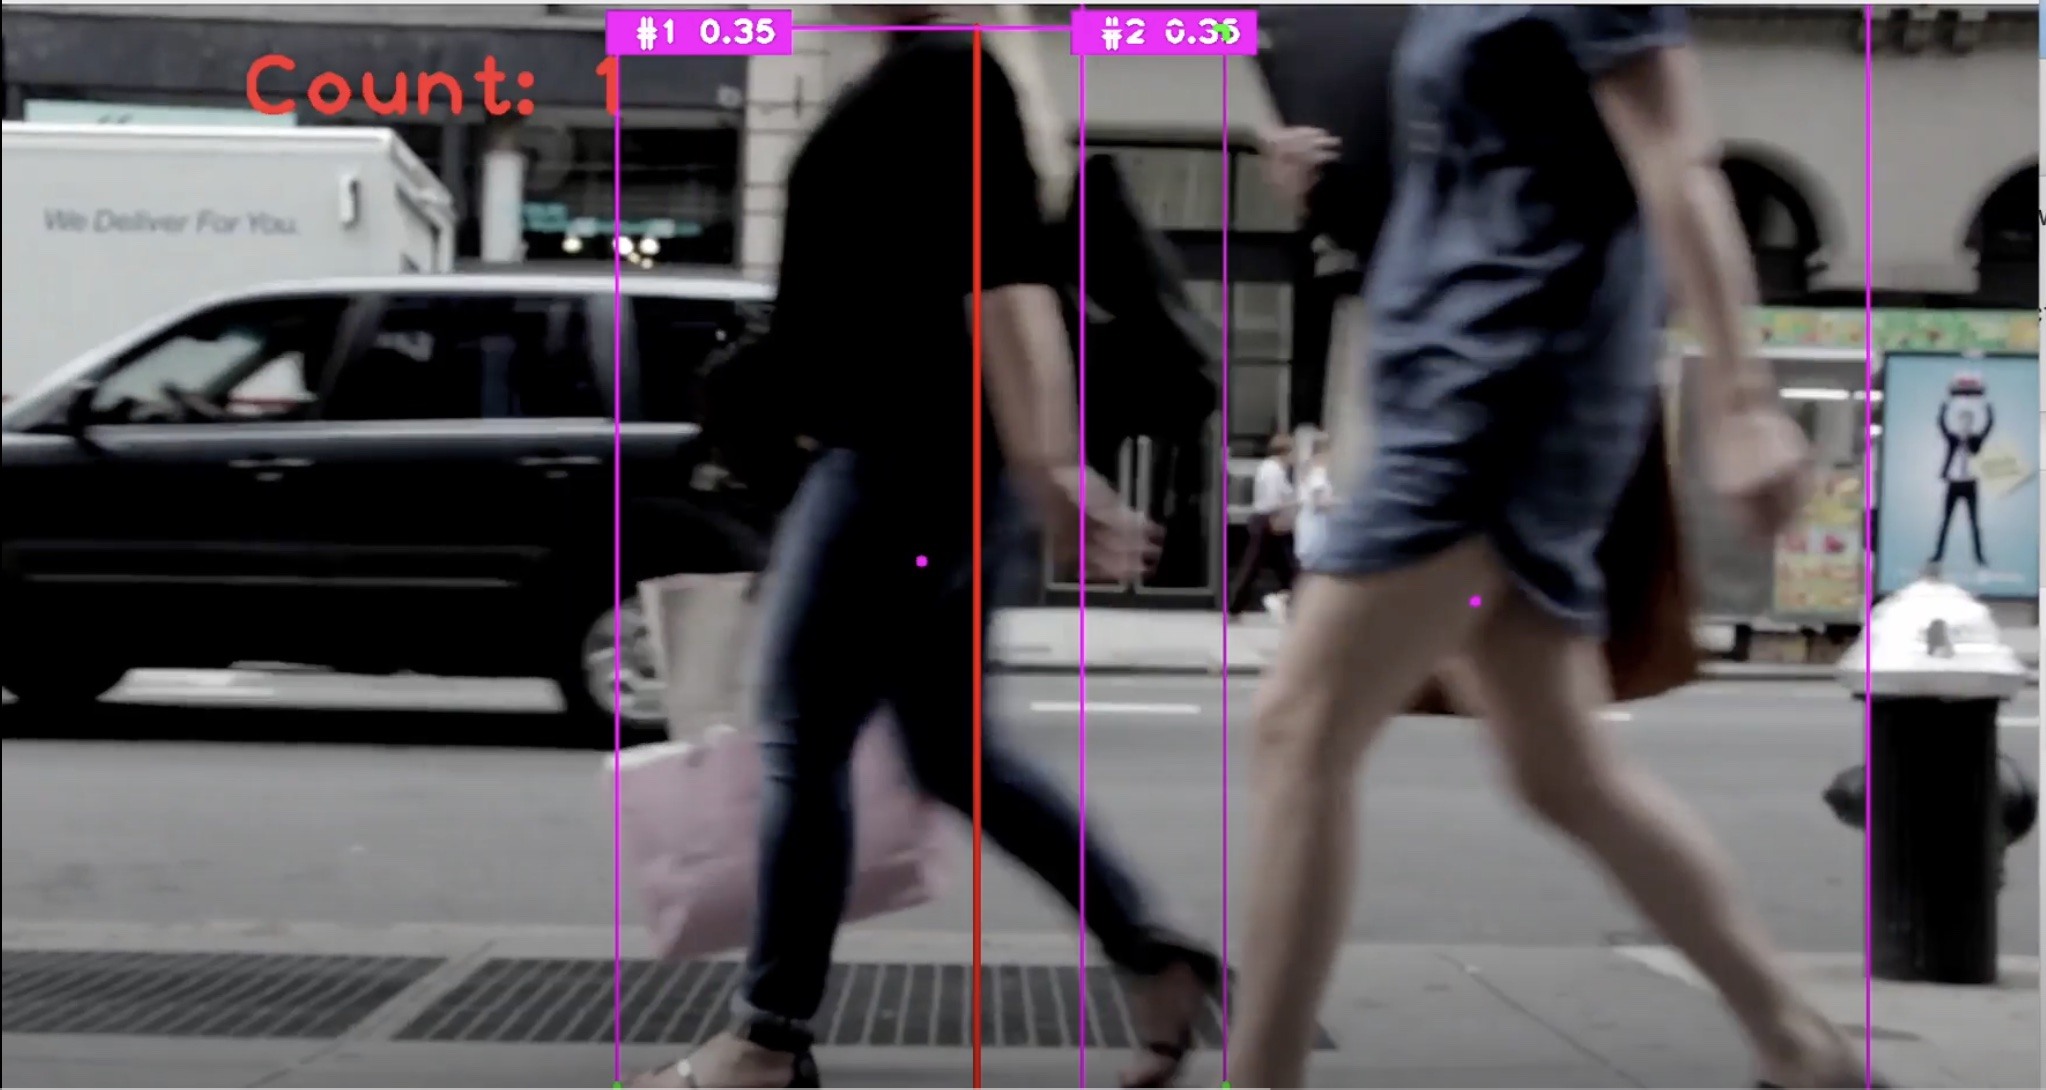
\includegraphics[width=0.5\textwidth]{Figures/Results/people counting.jpg}}
    \caption{People Detection and Counting.}
    \label{fig3c1}
\end{figure}

\begin{figure}[H]
    \centerline{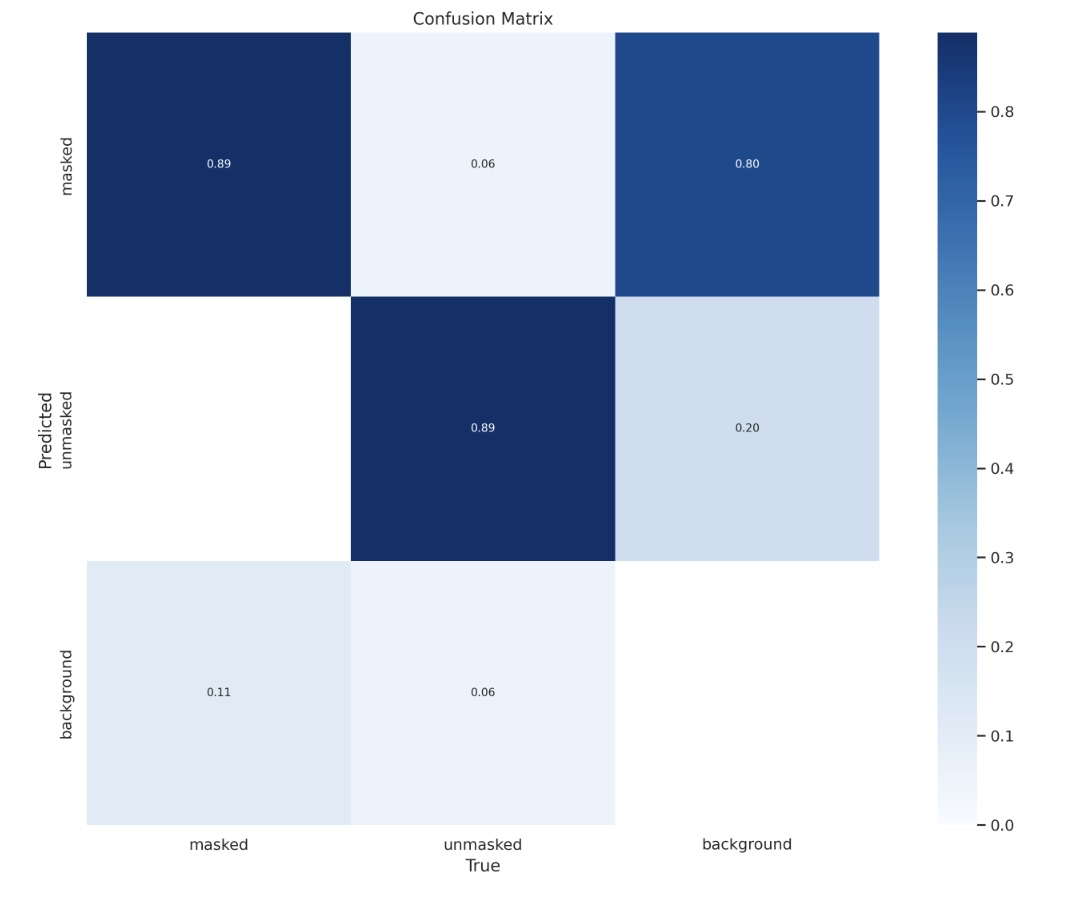
\includegraphics[width=0.5\textwidth]{Figures/Results/Confusion Matrix.jpg}}
    \caption{Confusion Matrix of Mask Detection Model.}
    \label{fig3c2}
\end{figure}

Fig.~\ref{fig3c1} shows the outcomes of the people counting function. Initially, individuals in each frame are identified by a red bounding box. YOLOv8 tracks these individuals and tallies them when the center of the bounding box intersects with a predefined line. For this specific experiment, the line is positioned at the center of the image.

Fig.~\ref{fig3c2} illustrates the performance metrics of the mask detection model. The achieved accuracy of this model is 89{\%}, indicating that individuals wearing masks can be correctly identified with an accuracy rate of 89{\%}.
\subsection{Software in the Loop (SITL)}

The SITL simulation conducted in this semester was showcased through a series of three experiments, each designed to test a specific aspect of the autonomous drone's capabilities. The first experiment focused on waypoint control, where waypoints were set with precise coordinates including position, altitude, and orientation utilizing set{\_}destination() function in the GNC library. The waypoints were designated as (5, 5), (15, 5), (15, -5), and (5, -5), with an altitude of 2 meters. At each waypoint, the orientations were set to 90, 180, 270, and 360 degrees, respectively. The drone successfully executed the task, initiating takeoff and then navigating to each waypoint in the prescribed sequence. A demonstration of a square flight trajectory with 4 waypoints is shown in Fig. \ref{fig3d1}. This outcome highlights the precision of the drone's flight path control and the efficacy of the GNC library.


\begin{figure}[H]
    \centerline{\includegraphics[width=0.5\textwidth]{Figures/Results/waypoints.jpeg}}
    \caption{Navigation through 4 Waypoints in Sequence (camera positioned vertically downward): 1 (top left) $\rightarrow$ 2 (top right) $\rightarrow$ 3 (bottom left) $\rightarrow$ 4 (bottom right)}
    \label{fig3d1}
\end{figure}

The second experiment evaluated the drone's human detection system. Four human models, featuring various genders and poses, were introduced into the simulation environment. To further challenge the system, interference objects were also added to the environment, simulating potential real-life distractions and occlusions that the drone might encounter. The OpenCV DNN module, equipped with the YOLO algorithm, was utilized to detect and count the number of humans in the frame. The experiment was successful as shown in Fig. \ref{fig3d2}. The system accurately identified and counted the human models, demonstrating the reliability of the object detection implementation.

\begin{figure}[H]
    \centerline{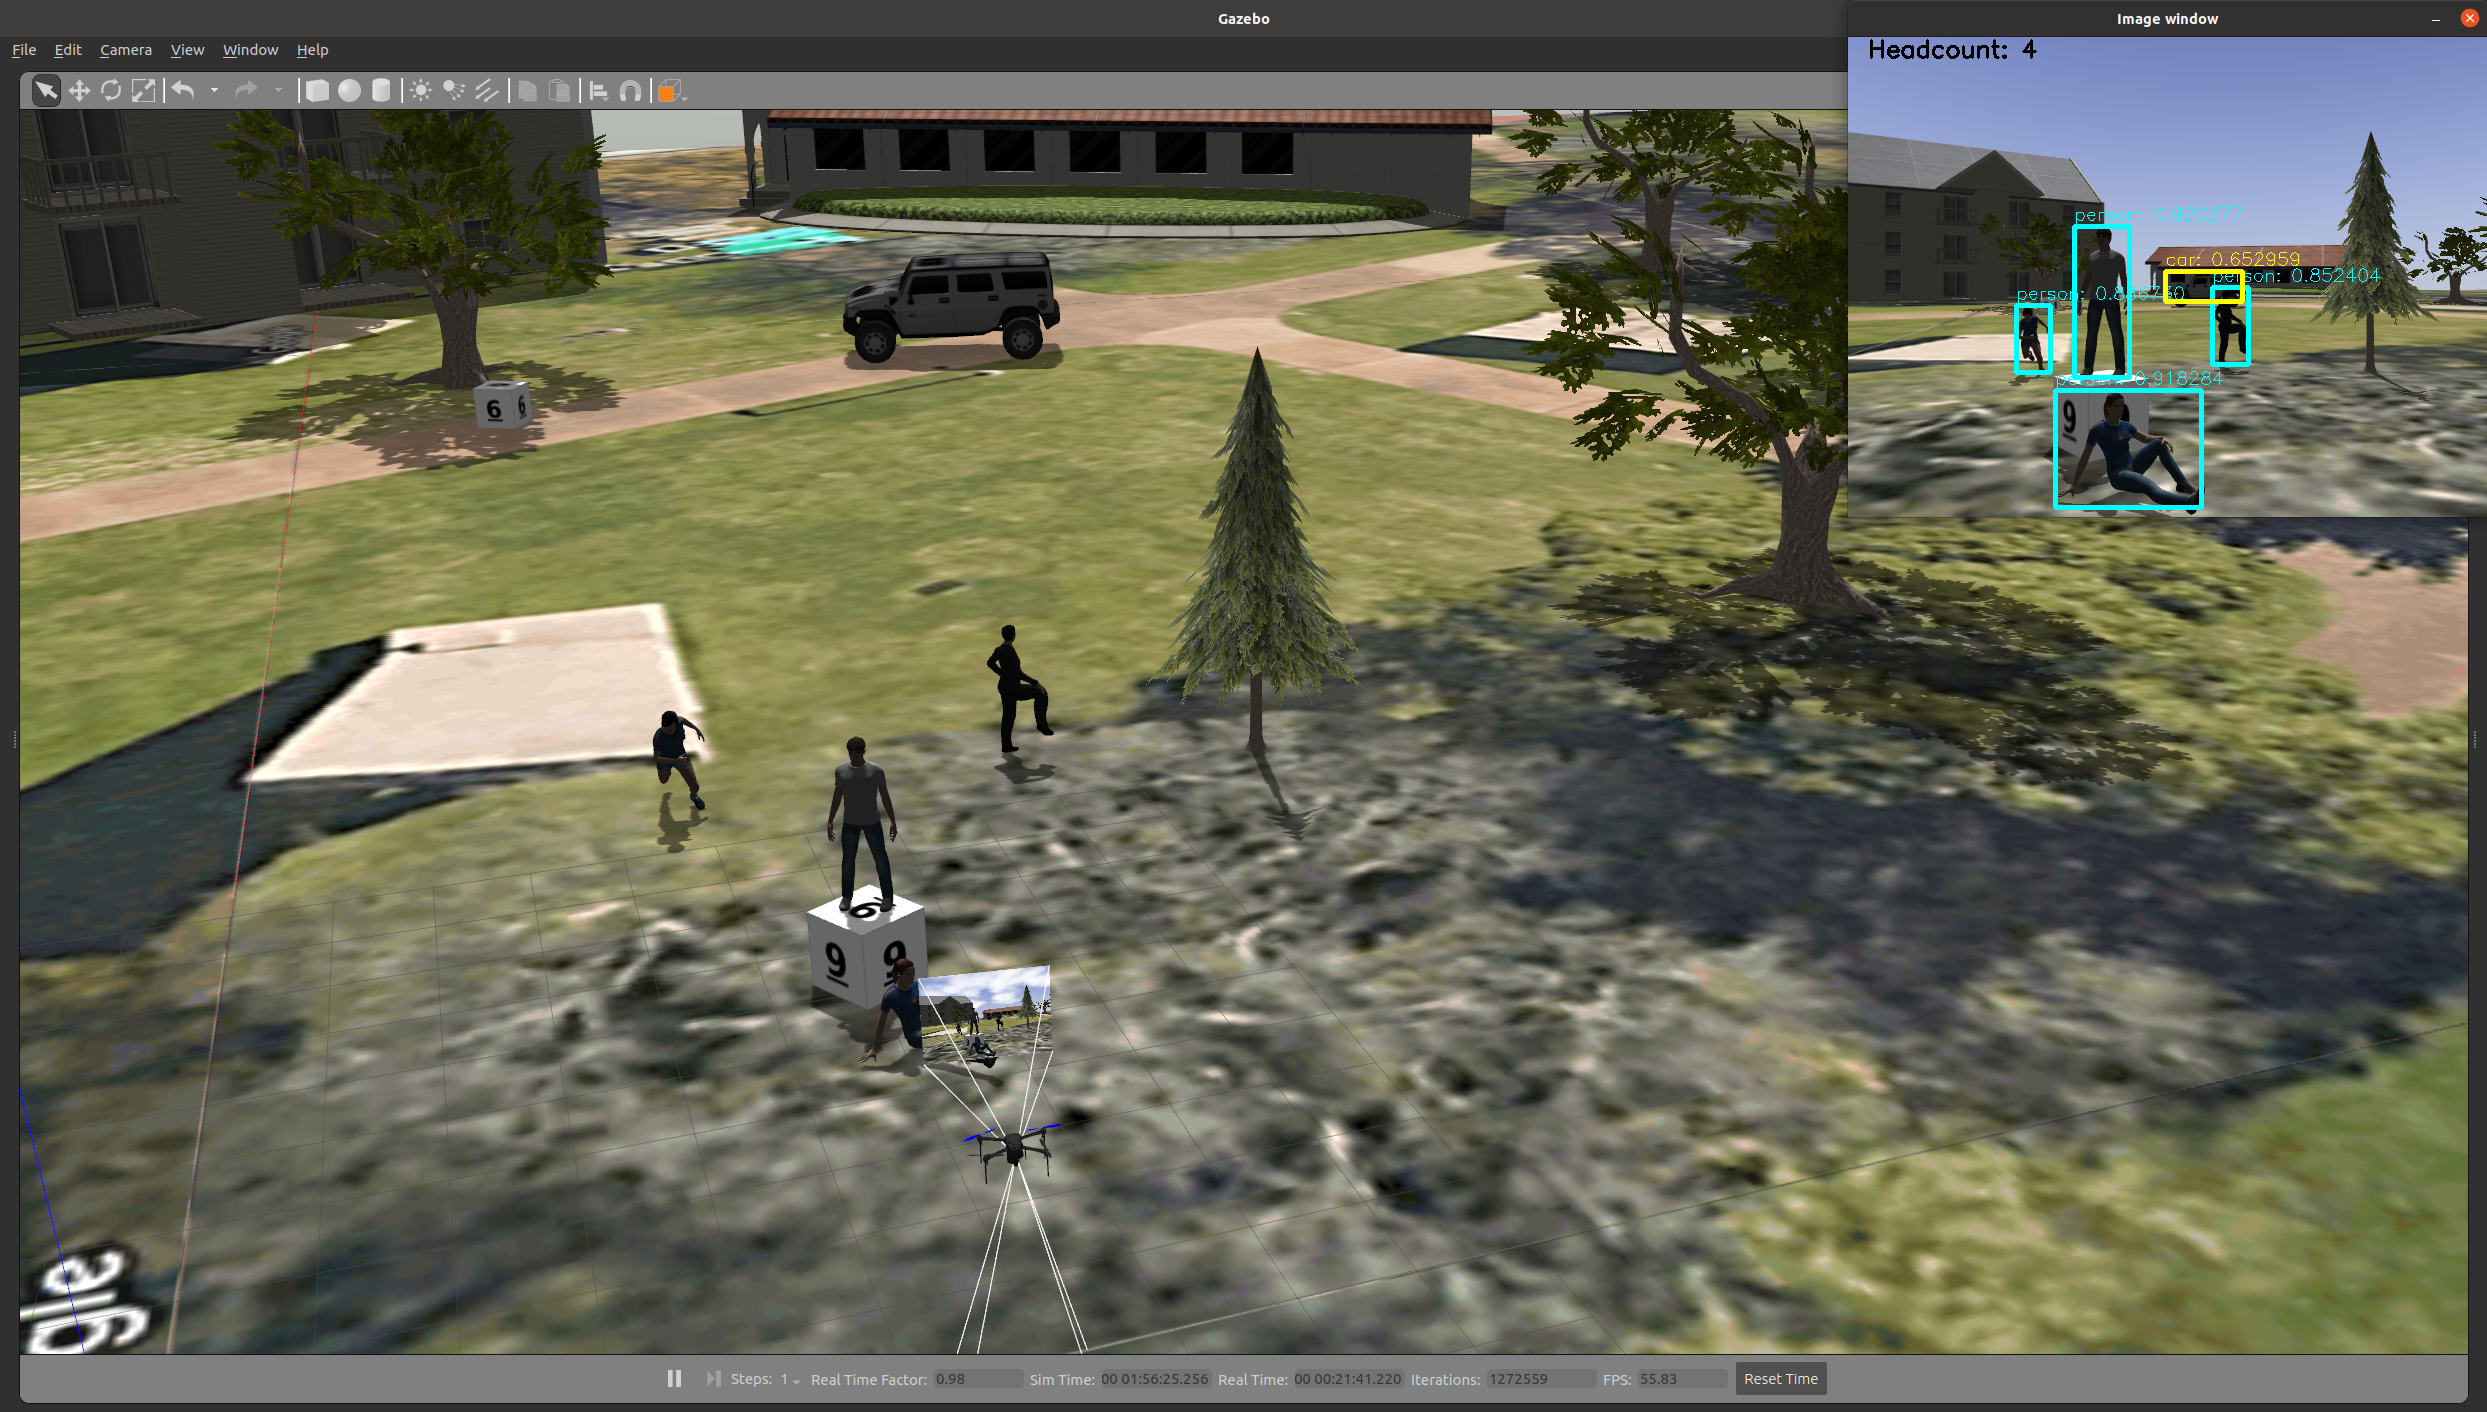
\includegraphics[width=0.5\textwidth]{Figures/Results/headcount.png}}
    \caption{Counting the Number of Humans in the Frame (camera positioned horizontally)}
    \label{fig3d2}
\end{figure}

The final experiment was designed to test the drone's capacity for dynamic human detection within its field of view. In this scenario, the drone was programmed to continuously rotate about its axis until it successfully detected a human model within its camera frame. The drone's software was programmed with algorithms to determine the human's relative position in the frame in real-time and adjust its orientation accordingly. As the drone began rotating, it utilized the integrated camera to scan the environment and processed the data with the YOLO model. The rotation speed was carefully calibrated to ensure sufficient time for image processing and recognition and balance between the agility of response and the accuracy of detection. A demonstration of the successful human tracking task is shown in Fig. \ref{fig3d3}. This result showcases the drone's advanced ability to autonomously identify and focus on human subjects in its environment.

\begin{figure}[H]
    \centerline{\includegraphics[width=0.5\textwidth]{Figures/Results/human_tracking.jpeg}}
    \caption{Human Tracking Task (camera positioned horizontally): Rotate (top left) $\rightarrow$ Rotate (top right) $\rightarrow$ Rotate (bottom left) $\rightarrow$ Stop (bottom right)}
    \label{fig3d3}
\end{figure}
\subsection{UI Interface}

From the system design diagram in Fig.~\ref{fig2b2}, it can be seen that we connect the Flight Controller to the SIK radio and then to the Mission Planner GUI of the computer, we follow this design to setup on the real drone system, the SIK Telemetry Radio devices on the left side of Fig.~\ref{fig2a2}, connected to the Cube Black Flight Controller's Telem Port 1, and the other one is connected to the Laptop's USB port, after initializing the settings in Mission Planner, you can successfully see the monitor screen as shown in Fig.~\ref{fig3e1}.

\begin{figure}[H]
    \centerline{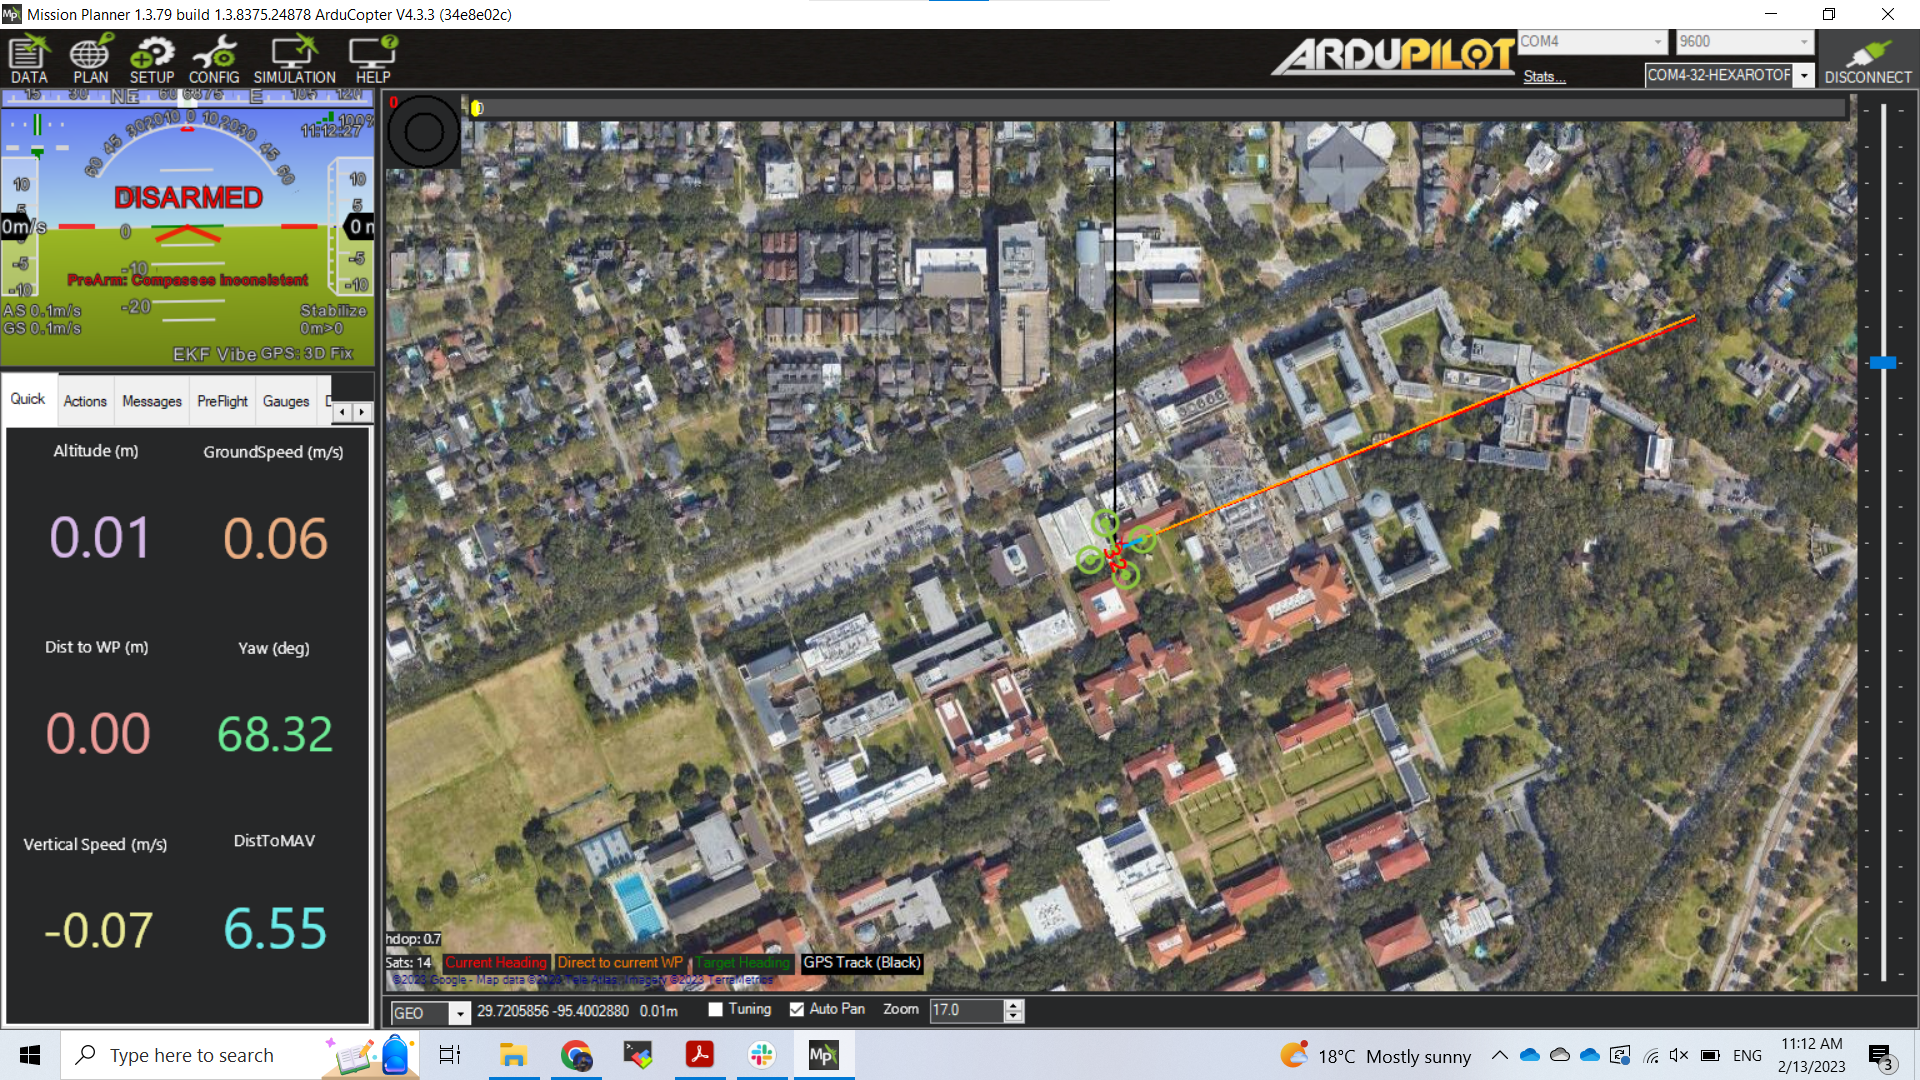
\includegraphics[width=0.5\textwidth]{Figures/Results/Mission_Planner_GUI.png}}
    \caption{Mission Planner GUI Interface.}
    \label{fig3e1}
\end{figure}

Fig.~\ref{fig3e2} shows the real-time status of the drone from SIK Telemetry Radio in Mission Planner GUI. The left side of the image shows the "DISARMED" status, which means the drone is not armed yet, and the right picture shows the "ARMED" status, which means the drone is armed and starts to spin the propellers at a fixed speed.

\begin{figure}[H]
    \centerline{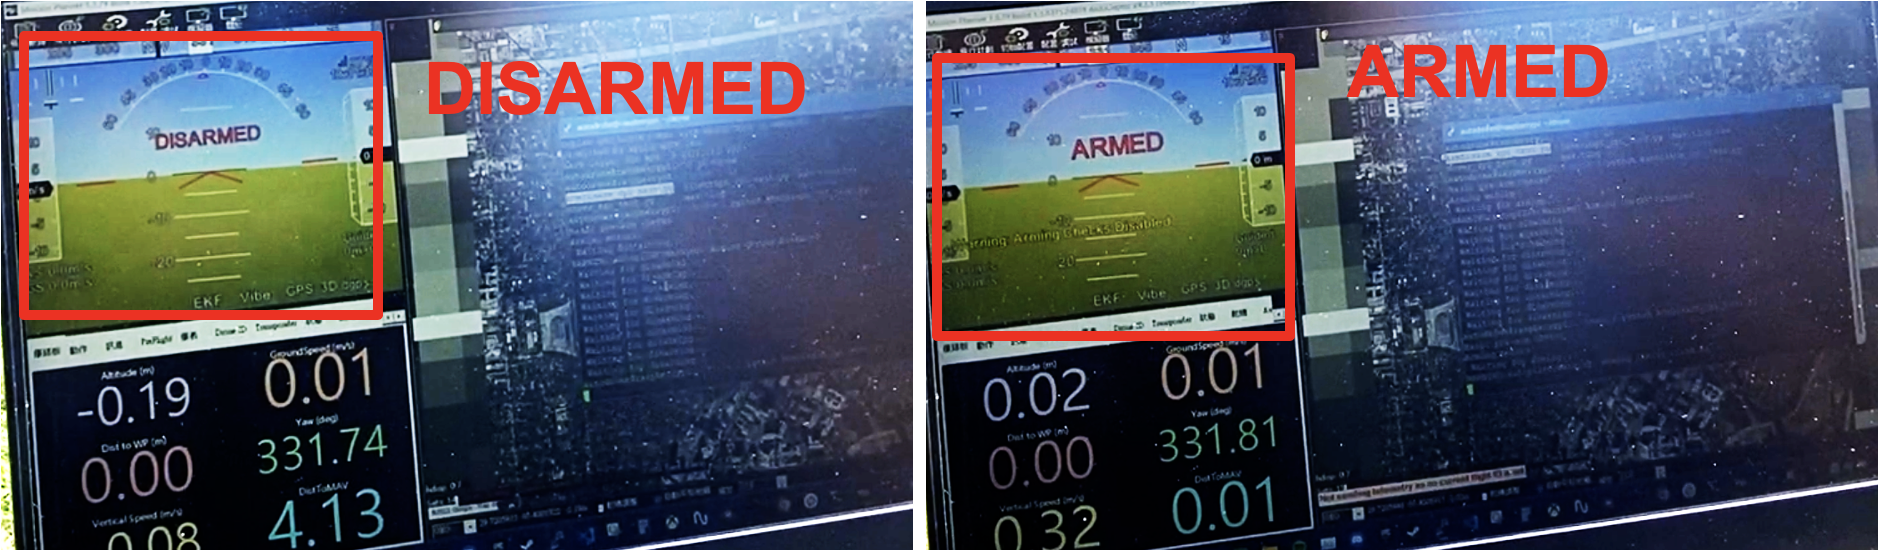
\includegraphics[width=0.5\textwidth]{Figures/Results/GUI_Status.png}}
    \caption{Drone's real-time status on Mission Planner GUI.}
    \label{fig3e2}
\end{figure}











\section{Discussion}

This semester's achievements in drone technology demonstrate remarkable progress, especially in hardware and software integration. The successful launch of the 4-axis plane with custom PCB is a testament to our ability in advanced UAV design and integration. Coupled with this, the implementation of Software In The Loop (SITL) for simultaneous object detection and drone control, along with the camera-LiDAR fusion, has significantly enhanced the drone's environmental awareness and operational efficiency. The application of the YOLOv8 model for mask detection further emphasizes our commitment to integrating cutting-edge AI into practical solutions.

% Challange
However, challenges still remain, particularly in achieving seamless integration and operational consistency across diverse environmental conditions. The complexity of real-world scenarios often presents unforeseen obstacles, such as variable lighting, unpredictable weather, and dynamic obstacles, which can affect the drone's performance. Moreover, ensuring consistent and reliable data processing from the fusion of camera and LiDAR inputs remains a technical challenge, requiring further refinement of our algorithms and sensor calibration methods. Another challenge is that the power consumption for the whole system is insufficient, causing the drone to shut down a few seconds after take off. Addressing these challenges will be crucial for advancing the drone's capabilities and ensuring its applicability in a wider range of scenarios.

% Future plan
Looking forward, the focus will be on enhancing the drone's autonomous functions and decision-making algorithms to tackle more complex tasks and adapt to changing environments. We aim to move from using the SITL simulation to testing with a real drone. A key goal is to make the drone use less power and fly longer distances, which might mean looking into new kinds of energy or better batteries. Adding more sensors and ways to communicate could also help the drone be used in more areas, like checking the environment or helping in emergencies. By continually developing and refining these systems, our team's objective is always to keep the drone technology advanced and reliable for a variety of uses.

\section*{Acknowledgment}

Repository for this project are available at: \url{https://github.com/Rice-MECE-Capstone-Projects/Autodrone} \\

Documents and tutorial for this project are available at: \url{https://riceautodrone.github.io/} \\

% \section*{References}

\begin{thebibliography}{00} 
\bibitem{1a1} Zhangqiang Ming, Min Zh, Xiangkun Wang, Jiamin Zhu, Junlong Cheng, Chengrui Gao, Yong Yang, Xiaoyong Wei, "Deep learning-based person re-identification methods: A survey and outlook of recent works", DOI:\url{https://ar5iv.labs.arxiv.org/html/2110.04764}

\bibitem{2c1} J. Redmon, S. Divvala, R. Girshick, A. Farhadi, ``You Only Look Once: Unified, Real-Time Object Detection,'' 2016 IEEE Conference on Computer Vision and Pattern Recognition (CVPR), May 2016, DOI: 10.1109/cvpr.2016.91.

\bibitem{2c2} G. Jocher et al., ultralytics/yolov5: v6.1 - TensorRT, TensorFlow Edge TPU and OpenVINO Export and Inference (v6.1). [Zenodo], 2022, DOI: 10.5281/zenodo.6222936.

\bibitem{2c3} Jocher, G., Chaurasia, A., Qiu, J. (2023). YOLO by Ultralytics (Version 8.0.0) [Computer software], DOI: \url{https://github.com/ultralytics/ultralytics}

\bibitem{2c4} Cabani, A., Hammoudi, K., Benhabiles, H., Melkemi, M. (2021), MaskedFace-Net – A dataset of correctly/incorrectly masked face images in the context of COVID-19. Smart Health, 19, 100144, DOI: \url{https://doi.org/10.1016/j.smhl.2020.100144}

\bibitem{2d1} RoboPeak Team. (2014). rplidar{\_}ros (Version master) [Computer software]. \url{https://github.com/Slamtec/rplidar_ros}

\bibitem{2e1} Gazebo Tutorials. (2023). Example World [Online tutorial]. \url{https://classic.gazebosim.org/tutorials?tut=static_map_plugin&cat=build_world#ExampleWorld}

\bibitem{2e2} Intelligent-Quads. (2023). iq{\_}gnc (Version master) [Computer software]. \url{https://github.com/Intelligent-Quads/iq_gnc/tree/master}


\end{thebibliography}
\vspace{12pt}



% \section{Methods}
Before you begin to format your paper, first write and save the content as a 
separate text file. Complete all content and organizational editing before 
formatting. Please note sections \ref{AA}--\ref{SCM} below for more information on 
proofreading, spelling and grammar.

Keep your text and graphic files separate until after the text has been 
formatted and styled. Do not number text heads---{\LaTeX} will do that 
for you.

\subsection{Abbreviations and Acronyms}\label{AA}
Define abbreviations and acronyms the first time they are used in the text, 
even after they have been defined in the abstract. Abbreviations such as 
IEEE, SI, MKS, CGS, ac, dc, and rms do not have to be defined. Do not use 
abbreviations in the title or heads unless they are unavoidable.

\subsection{Units}
\begin{itemize}
\item Use either SI (MKS) or CGS as primary units. (SI units are encouraged.) English units may be used as secondary units (in parentheses). An exception would be the use of English units as identifiers in trade, such as ``3.5-inch disk drive''.
\item Avoid combining SI and CGS units, such as current in amperes and magnetic field in oersteds. This often leads to confusion because equations do not balance dimensionally. If you must use mixed units, clearly state the units for each quantity that you use in an equation.
\item Do not mix complete spellings and abbreviations of units: ``Wb/m\textsuperscript{2}'' or ``webers per square meter'', not ``webers/m\textsuperscript{2}''. Spell out units when they appear in text: ``. . . a few henries'', not ``. . . a few H''.
\item Use a zero before decimal points: ``0.25'', not ``.25''. Use ``cm\textsuperscript{3}'', not ``cc''.)
\end{itemize}

\subsection{Equations}
Number equations consecutively. To make your 
equations more compact, you may use the solidus (~/~), the exp function, or 
appropriate exponents. Italicize Roman symbols for quantities and variables, 
but not Greek symbols. Use a long dash rather than a hyphen for a minus 
sign. Punctuate equations with commas or periods when they are part of a 
sentence, as in:
\begin{equation}
a+b=\gamma\label{eq}
\end{equation}

Be sure that the 
symbols in your equation have been defined before or immediately following 
the equation. Use ``\eqref{eq}'', not ``Eq.~\eqref{eq}'' or ``equation \eqref{eq}'', except at 
the beginning of a sentence: ``Equation \eqref{eq} is . . .''

\subsection{\LaTeX-Specific Advice}

Please use ``soft'' (e.g., \verb|\eqref{Eq}|) cross references instead
of ``hard'' references (e.g., \verb|(1)|). That will make it possible
to combine sections, add equations, or change the order of figures or
citations without having to go through the file line by line.

Please don't use the \verb|{eqnarray}| equation environment. Use
\verb|{align}| or \verb|{IEEEeqnarray}| instead. The \verb|{eqnarray}|
environment leaves unsightly spaces around relation symbols.

Please note that the \verb|{subequations}| environment in {\LaTeX}
will increment the main equation counter even when there are no
equation numbers displayed. If you forget that, you might write an
article in which the equation numbers skip from (17) to (20), causing
the copy editors to wonder if you've discovered a new method of
counting.

{\BibTeX} does not work by magic. It doesn't get the bibliographic
data from thin air but from .bib files. If you use {\BibTeX} to produce a
bibliography you must send the .bib files. 

{\LaTeX} can't read your mind. If you assign the same label to a
subsubsection and a table, you might find that Table I has been cross
referenced as Table IV-B3. 

{\LaTeX} does not have precognitive abilities. If you put a
\verb|\label| command before the command that updates the counter it's
supposed to be using, the label will pick up the last counter to be
cross referenced instead. In particular, a \verb|\label| command
should not go before the caption of a figure or a table.

Do not use \verb|\nonumber| inside the \verb|{array}| environment. It
will not stop equation numbers inside \verb|{array}| (there won't be
any anyway) and it might stop a wanted equation number in the
surrounding equation.

\subsection{Some Common Mistakes}\label{SCM}
\begin{itemize}
\item The word ``data'' is plural, not singular.
\item The subscript for the permeability of vacuum $\mu_{0}$, and other common scientific constants, is zero with subscript formatting, not a lowercase letter ``o''.
\item In American English, commas, semicolons, periods, question and exclamation marks are located within quotation marks only when a complete thought or name is cited, such as a title or full quotation. When quotation marks are used, instead of a bold or italic typeface, to highlight a word or phrase, punctuation should appear outside of the quotation marks. A parenthetical phrase or statement at the end of a sentence is punctuated outside of the closing parenthesis (like this). (A parenthetical sentence is punctuated within the parentheses.)
\item A graph within a graph is an ``inset'', not an ``insert''. The word alternatively is preferred to the word ``alternately'' (unless you really mean something that alternates).
\item Do not use the word ``essentially'' to mean ``approximately'' or ``effectively''.
\item In your paper title, if the words ``that uses'' can accurately replace the word ``using'', capitalize the ``u''; if not, keep using lower-cased.
\item Be aware of the different meanings of the homophones ``affect'' and ``effect'', ``complement'' and ``compliment'', ``discreet'' and ``discrete'', ``principal'' and ``principle''.
\item Do not confuse ``imply'' and ``infer''.
\item The prefix ``non'' is not a word; it should be joined to the word it modifies, usually without a hyphen.
\item There is no period after the ``et'' in the Latin abbreviation ``et al.''.
\item The abbreviation ``i.e.'' means ``that is'', and the abbreviation ``e.g.'' means ``for example''.
\end{itemize}
An excellent style manual for science writers is \cite{b7}.

\subsection{Authors and Affiliations}
\textbf{The class file is designed for, but not limited to, six authors.} A 
minimum of one author is required for all conference articles. Author names 
should be listed starting from left to right and then moving down to the 
next line. This is the author sequence that will be used in future citations 
and by indexing services. Names should not be listed in columns nor group by 
affiliation. Please keep your affiliations as succinct as possible (for 
example, do not differentiate among departments of the same organization).

\subsection{Identify the Headings}
Headings, or heads, are organizational devices that guide the reader through 
your paper. There are two types: component heads and text heads.

Component heads identify the different components of your paper and are not 
topically subordinate to each other. Examples include Acknowledgments and 
References and, for these, the correct style to use is ``Heading 5''. Use 
``figure caption'' for your Figure captions, and ``table head'' for your 
table title. Run-in heads, such as ``Abstract'', will require you to apply a 
style (in this case, italic) in addition to the style provided by the drop 
down menu to differentiate the head from the text.

Text heads organize the topics on a relational, hierarchical basis. For 
example, the paper title is the primary text head because all subsequent 
material relates and elaborates on this one topic. If there are two or more 
sub-topics, the next level head (uppercase Roman numerals) should be used 
and, conversely, if there are not at least two sub-topics, then no subheads 
should be introduced.

\subsection{Figures and Tables}
\paragraph{Positioning Figures and Tables} Place figures and tables at the top and 
bottom of columns. Avoid placing them in the middle of columns. Large 
figures and tables may span across both columns. Figure captions should be 
below the figures; table heads should appear above the tables. Insert 
figures and tables after they are cited in the text. Use the abbreviation 
``Fig.~\ref{fig}'', even at the beginning of a sentence.

\begin{table}[htbp]
\caption{Table Type Styles}
\begin{center}
\begin{tabular}{|c|c|c|c|}
\hline
\textbf{Table}&\multicolumn{3}{|c|}{\textbf{Table Column Head}} \\
\cline{2-4} 
\textbf{Head} & \textbf{\textit{Table column subhead}}& \textbf{\textit{Subhead}}& \textbf{\textit{Subhead}} \\
\hline
copy& More table copy$^{\mathrm{a}}$& &  \\
\hline
\multicolumn{4}{l}{$^{\mathrm{a}}$Sample of a Table footnote.}
\end{tabular}
\label{tab1}
\end{center}
\end{table}

\begin{figure}[htbp]
\centerline{
\includegraphics{fig1.png}}
\caption{Example of a figure caption.}
\label{fig}
\end{figure}

Figure Labels: Use 8 point Times New Roman for Figure labels. Use words 
rather than symbols or abbreviations when writing Figure axis labels to 
avoid confusing the reader. As an example, write the quantity 
``Magnetization'', or ``Magnetization, M'', not just ``M''. If including 
units in the label, present them within parentheses. Do not label axes only 
with units. In the example, write ``Magnetization (A/m)'' or ``Magnetization 
\{A[m(1)]\}'', not just ``A/m''. Do not label axes with a ratio of 
quantities and units. For example, write ``Temperature (K)'', not 
``Temperature/K''.


\end{document}
